%% abtex2-modelo-trabalho-academico.tex, v-1.9.6 laurocesar
%% Copyright 2012-2016 by abnTeX2 group at http://www.abntex.net.br/ 
%%
%% This work may be distributed and/or modified under the
%% conditions of the LaTeX Project Public License, either version 1.3
%% of this license or (at your option) any later version.
%% The latest version of this license is in
%%   http://www.latex-project.org/lppl.txt
%% and version 1.3 or later is part of all distributions of LaTeX
%% version 2005/12/01 or later.
%%
%% This work has the L PPL maintenance status `maintained'.
%% 
%% The Current Maintainer of this work is the abnTeX2 team, led
%% by Lauro César Araujo. Further information are available on 
%% http://www.abntex.net.br/
%%
%% This work consists of the files abntex2-modelo-trabalho-academico.tex,
%% abntex2-modelo-include-comandos and abntex2-modelo-references.bib
% ------------------------------------------------------------------------
% ------------------------------------------------------------------------
% abnTeX2: Modelo de Trabalho Academico (tese de doutorado, dissertacao de
% mestrado e trabalhos monograficos em geral) em conformidade com 
% ABNT NBR 14724:2011: Informacao e documentacao - Trabalhos academicos -
% Apresentacao
% ------------------------------------------------------------------------
% ------------------------------------------------------------------------
% Personalização para o modelo Udesc 2024 9. ed. revisada e modificada
% Manual_13_05_2024_17175220258266_12510.pdf acesso em: 13/08/2024
% Autor: Felipe Joel Zimann (felipezimann@hotmail.com)
% Data: 02/12/2020 v1.0
% Data: 13/02/2021 v1.0.1 alterado tamanho numeração da página para 10pt
% Data: 13/08/2024 v1.0.2 alterado para citação (Autor, Ano) ao invés de (AUTOR, Ano) conforme ABNT NBR 10520:2023
% ------------------------------------------------------------------------
% ------------------------------------------------------------------------

\documentclass[
	12pt,					% tamanho da fonte
	openright,				% capítulos começam em pág ímpar (insere página vazia caso preciso)
	oneside,				% para impressão em recto e verso (twoside). Oposto a (oneside)
	a4paper,				% tamanho do papel. 
	chapter=TITLE,			% títulos de capítulos convertidos em letras maiúsculas
	section=TITLE,			% títulos de seções convertidos em letras maiúsculas
	sumario=abnt-6027-2012,
	english,				% idioma adicional para hifenização
	brazil,					% o último idioma é o principal do documento
	fleqn,					% equações alinhadas a esquerda (UDESC/CCT)+
	]{abntex2}

% ----------------------------------------------------------
% Pacotes básicos 
% ----------------------------------------------------------
\usepackage{amsmath}							% Pacote matemático
\usepackage{amssymb}							% Pacote matemático
\usepackage{amsfonts}							% Pacote matemático
%\usepackage{lmodern}							% Usa a fonte Latin Modern		
\usepackage{mathptmx} 							% Usa a fonte Times New Roman	 (UDESC/CCT)
\usepackage[T1]{fontenc}						% Selecao de codigos de fonte.
\usepackage[utf8]{inputenc}						% Codificacao do documento (conversão automática dos acentos)
\usepackage{lastpage}							% Usado pela Ficha catalográfica
\usepackage{indentfirst}						% Indenta o primeiro parágrafo de cada seção.
\usepackage[dvipsnames,table]{xcolor}			% Controle das cores
\usepackage{graphicx}							% Inclusão de gráficos
\usepackage{microtype} 							% para melhorias de justificação
\usepackage{lipsum}								% para geração de dummy text
\usepackage[brazilian,hyperpageref]{backref}	% Paginas com as citações na bibl
\usepackage[alf,abnt-emphasize=bf,abnt-full-initials=yes]{abntex2cite}
\usepackage{booktabs}
\usepackage{url} % se ainda não estiver ativo
\citeoption{abnt-url-package=url}

%\usepackage[num]{abntex2cite}					% Citações padrão ABNT numérica
\usepackage{adjustbox}							% Pacote de ajuste de boxes
\usepackage{subcaption}							% Inclusão de Subfiguras e sublegendas		
\usepackage{enumitem}							% Personalização de listas
\usepackage{siunitx}							% Grandezas e unidades
\usepackage[section]{placeins}					% Manter as figuras delimitadas na respectiva seção com a opção [section]
\usepackage{multirow}							% Multi colunas nas tabelas
\usepackage{array,tabularx} 					% Pacotes de tabelas
\usepackage{rotating}							% Rotacionar figuras e tabelas
\usepackage{xfrac}								% Fazer frações n/d em linha
\usepackage{bm}									% Negrito em modo matemático
\usepackage{xstring}							% Manipulação de strings
\usepackage{pgfplots}							% Pacote de Gráficos
\usepackage{tikz}								% Pacote de Figuras
\usepackage[american, cuteinductors,smartlabels, fulldiode, siunitx, americanvoltages, oldvoltagedirection, smartlabels]{circuitikz}						% Pacote de circuitos elétricos
\usepackage{chemformula}						% Pacote para fórmulas químicas
\usepackage{chngcntr}							% Pacte usado para deixar numeração de equações sequencial (UDESC/CCT)
\usepackage{caption}
\usepackage{makecell} % Add this line at the beginning of the document
\usepackage{array}
\usepackage{ragged2e}
\usepackage{pdflscape}
\usepackage{threeparttable}
\usepackage{threeparttablex}
\usepackage{ltablex}
\usepackage{csvsimple}    % lê CSV
\usepackage{booktabs}     % linhas bonitas
\usepackage{longtable}    % tabelas que quebram página
% \usepackage{float}
\counterwithout{equation}{chapter}
% fonte: https://latex.org/forum/viewtopic.php?t=15392

% Comando para deixar numeração das equações contínua (1), (2), (3)... ao invés de organizar por capítulos (1.1)(1.2)... (2.1)(2.2)
%\renewcommand{\theequation}{\arabic{equation}}

%\numberwithin{equation}{section}

\usepackage[utf8]{inputenc}
\usepackage[T1]{fontenc}
\DeclareUnicodeCharacter{2212}{\ensuremath{-}} % “−” → sinal de menos
\DeclareUnicodeCharacter{2013}{--}             % “–” → en-dash

% depois de babel[brazilian] e hyperref
\addto\extrasbrazilian{%
  \renewcommand{\sectionautorefname}{Seção}%
  \renewcommand{\subsectionautorefname}{Seção}%
  \renewcommand{\appendixname}{Apêndice}%
  \renewcommand{\tableautorefname}{Tabela}%
  \renewcommand{\figureautorefname}{Figura}%
}

\newcommand{\notafig}{\newline Fonte: elaboração do autor com base nos modelos da \autoref{sec:modelo-estatistico} (contrafactual da \autoref{sec:publico_esclarecido})}%


% Cabecalho cabeçalho somente com numeração de página 10pt
\makepagestyle{PagNumReduzida}
\makeevenhead{PagNumReduzida}{\ABNTEXfontereduzida\thepage}{}{}
\makeoddhead{PagNumReduzida}{}{}{\ABNTEXfontereduzida\thepage}
%fonte: https://github.com/abntex/abntex2/wiki/HowToCustomizarCabecalhoRodape
%fonte: Manual memoir seção 7.3 pg. 111 pdf http://linorg.usp.br/CTAN/macros/latex/contrib/memoir/memman.pdf 

% Personalização das opções das listas
\setlist[itemize]{leftmargin=\parindent}

% Citação online --- MODIFICAR ---
\newcommand{\citeshort}[1]{\citeauthoronline{#1}~(\citeyear{#1})}

\newcommand{\me}[1]{Elaborado pelo autor (#1).}

% Configuração do pgfplots
\pgfplotsset{compat=newest} %compat=1.14
\pgfplotsset{plot coordinates/math parser=false} 
\newlength\figureheight 
\newlength\figurewidth 

% Libraries do TiKz
\usetikzlibrary{quotes,angles,arrows}
\usetikzlibrary{through,calc,math}
\usetikzlibrary{graphs,backgrounds,fit}
\usetikzlibrary{shapes,positioning,patterns,shadows}
\usetikzlibrary{decorations.pathreplacing}
\usetikzlibrary{shapes.geometric}
\usetikzlibrary{arrows.meta}
\usetikzlibrary{external}

%\tikzexternalize[]
%\tikzexternalenable
%\tikzexternalize
%\tikzexternaldisable
%\tikzset{external/force remake}
%\tikzexternalize[shell escape=-enable-write18]

% Configurações do CircuiTiKz
\ctikzset{bipoles/thickness=1}
%\ctikzset{bipoles/length=1.2cm}
\ctikzset{monopoles/ground/width/.initial=.2}
\ctikzset{bipoles/resistor/height=0.25}
\ctikzset{bipoles/resistor/width=0.6}
\ctikzset{bipoles/capacitor/height=0.5}
\ctikzset{bipoles/capacitor/width=0.15}
\ctikzset{bipoles/generic/height=0.25}
\ctikzset{bipoles/generic/width=0.6}
%\ctikzset{bipoles/capacitor polar/length=0.5}
%\ctikzset{bipoles/diode/height=.375}
%\ctikzset{bipoles/diode/width=.3}
%\ctikzset{tripoles/thyristor/height=.8}
%\ctikzset{tripoles/thyristor/width=1}
\ctikzset{bipoles/vsourcesin/height=.5}
\ctikzset{bipoles/vsourcesin/width=.5}
\ctikzset{bipoles/cvsourceam/height=.6}
\ctikzset{bipoles/cvsourceam/width=.6}
%\ctikzset{tripoles/european controlled voltage source/width=.4}

\tikzstyle{every node}=[font=\footnotesize]
\tikzstyle{every path}=[line width=0.25pt,line cap=round,line join=round]
%\tikzstyle{every path}=[line cap=round,line join=round]


% Definição de cores MATLAB
\definecolor{matlab_blue}{rgb}	{         0,    0.4470,    0.7410}
\definecolor{matlab_orange}{rgb}{    0.8500,    0.3250,    0.0980}
\definecolor{matlab_yellow}{rgb}{    0.9290,    0.6940,    0.1250}
\definecolor{matlab_violet}{rgb}{    0.4940,    0.1840,    0.5560}
\definecolor{matlab_green}{rgb}	{	 0.4660,    0.6740,    0.1880}
\definecolor{matlab_lblue}{rgb}	{    0.3010,    0.7450,    0.9330}
\definecolor{matlab_red}{rgb}	{    0.6350,    0.0780,    0.1840}

% Personalização das legendas
\usepackage[format = plain, %hang
			justification = centering,
			labelsep = endash,
			singlelinecheck = false,
			skip = 6pt,
			listformat = simple]{caption}	

% Personalização das unidades
\sisetup{output-decimal-marker = {,}}
\sisetup{exponent-product = \cdot}
\sisetup{tight-spacing=true}
\sisetup{group-digits = false}

% Personalizações de tipo de colunas de tabelas
\newcolumntype{L}[1]{>{\raggedright\let\newline\\\arraybackslash\hspace{0pt}}m{#1}}
\newcolumntype{C}[1]{>{\centering\let\newline\\\arraybackslash\hspace{0pt}}m{#1}}
\newcolumntype{R}[1]{>{\raggedleft\let\newline\\\arraybackslash\hspace{0pt}}m{#1}}

% Personalizações de cores da UDESC
\definecolor{CapaAmareloUDESC}{RGB}{243,186,83}		% Especializacao
\definecolor{CapaVerdeUDESC}{RGB}{0,112,52}			% Mestrado
\definecolor{CapaVermelhoUDESC}{RGB}{171,35,21}		% Doutorado
\definecolor{CapaAzulUDESC}{RGB}{38,54,118} 		% Pós-Doutorado

% CONFIGURAÇÕES DE PACOTES
% Configurações do pacote backref
% Usado sem a opção hyperpageref de backref
\renewcommand{\backrefpagesname}{}
% \renewcommand{\backrefpagesname}{Citado na(s) página(s):~}
% Texto padrão antes do número das páginas
\renewcommand{\backref}{}
% Define os textos da citação
% \renewcommand*{\backrefalt}[4]{
% 	\ifcase #1 %
% 	Nenhuma citação no texto.%
% 	\or
% 	Citado na página #2.%
% 	\else
% 	Citado #1 vezes nas páginas #2.%
% 	\fi}%

\renewcommand*{\backrefalt}[4]{}%

% alterando o aspecto da cor azul
%\definecolor{blue}{RGB}{41,5,195}

% informações do PDF
\makeatletter
\hypersetup{
	%pagebackref=true,
	pdftitle={\@title}, 
	pdfauthor={\@author},
	pdfsubject={\imprimirpreambulo},
	pdfcreator={LaTeX with abnTeX2},
	pdfkeywords={abnt}{latex}{abntex}{abntex2}{trabalho academico}, 
	colorlinks=true,       		% false: boxed links; true: colored links
	linkcolor=black,          	% color of internal links
	citecolor=black,        	% color of links to bibliography
	filecolor=black,      		% color of file links
	urlcolor=black,
	bookmarksdepth=4
}
\makeatother


\makeatletter
\newcommand{\includetikz}[1]{%
	\tikzsetnextfilename{#1}%
	\input{#1.tex}%
}
\makeatother


% ---
% Possibilita criação de Quadros e Lista de quadros.
% Ver https://github.com/abntex/abntex2/issues/176
%
\newcommand{\quadroname}{Quadro}
\newcommand{\listofquadrosname}{Lista de quadros}

\newfloat[chapter]{quadro}{loq}{\quadroname}
\newlistof{listofquadros}{loq}{\listofquadrosname}
\newlistentry{quadro}{loq}{0}

% configurações para atender às regras da ABNT
\setfloatadjustment{quadro}{\centering}
\counterwithout{quadro}{chapter}
\renewcommand{\cftquadroname}{\quadroname\space} 
\renewcommand*{\cftquadroaftersnum}{\hfill--\hfill}

\setfloatlocations{quadro}{hbtp} % Ver https://github.com/abntex/abntex2/issues/176
% ---


% Espaçamento depois do título
\setlength{\afterchapskip}{0.7\baselineskip}
% O tamanho do parágrafo é dado por:
\setlength{\parindent}{1.25cm}
% Controle do espaçamento entre um parágrafo e outro:
\setlength{\parskip}{0.0cm}  % tente também \onelineskip
%\SingleSpacing % Espaçamento simples 
\OnehalfSpacing % Espaçamento 1,5 (UDESC/CCT)
%\DoubleSpacing	% Espaçamento duplo

% ---
% Margens - NBR 14724/2011 - 5.1 Formato
% ---
\setlrmarginsandblock{3cm}{2cm}{*}
\setulmarginsandblock{3cm}{2cm}{*}
\checkandfixthelayout[fixed]
% ---


% To use externalize consider
%https://tex.stackexchange.com/questions/182783/tikzexternalize-not-compatible-with-miktex-2-9-abntex2-package
%Lauro Cesar digged into the problem until he came with a solution for me to test. And it Works!
%
%According to this link:
%
%The package calc changed the commands \setcounter and friends to be fragile. So you have to make them robust. The example below uses etoolbox with \robustify:
%
\usepackage{etoolbox}
\robustify\setcounter
\robustify\addtocounter
\robustify\setlength
\robustify\addtolength


%% How to silence memoir class warning against the use of caption package?
%% https://tex.stackexchange.com/questions/391993/how-to-silence-memoir-class-warning-against-the-use-of-caption-package
%\usepackage{silence}
%\WarningFilter*{memoir}{You are using the caption package with the memoir class}
%\WarningFilter*{Class memoir Warning}{You are using the caption package with the memoir class}

% --------------------------------------------------------
% INICIO DAS CUSTOMIZACOES PARA A UDESC
% --------------------------------------------------------

% --------------------------------------------------------
% Fontes padroes de part, chapter, section, subsection e subsubsection
% --------------------------------------------------------
% --- Chapter ---
\renewcommand{\ABNTEXchapterfont}{\fontseries{b}} %\bfseries
\renewcommand{\ABNTEXchapterfontsize}{\normalsize}
% --- Part ---
\renewcommand{\ABNTEXpartfont}{\ABNTEXchapterfont}
\renewcommand{\ABNTEXpartfontsize}{\LARGE}
% --- Section ---
\renewcommand{\ABNTEXsectionfont}{\normalfont}
\renewcommand{\ABNTEXsectionfontsize}{\normalsize}
% --- SubSection ---
\renewcommand{\ABNTEXsubsectionfont}{\fontseries{b}} %\bfseries
\renewcommand{\ABNTEXsubsectionfontsize}{\normalsize}
% --- SubSubSection ---
\renewcommand{\ABNTEXsubsubsectionfont}{\itshape}
\renewcommand{\ABNTEXsubsubsectionfontsize}{\normalsize}

\renewcommand{\ABNTEXsubsubsubsectionfont}{\normalfont}
\renewcommand{\ABNTEXsubsubsubsectionfontsize}{\normalsize}
% ---

% --------------------------------------------------------
% Fontes das entradas do sumario
% --------------------------------------------------------

\renewcommand{\cftpartfont}{\ABNTEXpartfont\selectfont}
\renewcommand{\cftpartpagefont}{\normalsize\selectfont}

\renewcommand{\cftchapterfont}{\ABNTEXchapterfont\selectfont}
\renewcommand{\cftchapterpagefont}{\normalsize\selectfont}

\renewcommand{\cftsectionfont}{\ABNTEXsectionfont\selectfont}
\renewcommand{\cftsectionpagefont}{\normalsize\selectfont}

\renewcommand{\cftsubsectionfont}{\ABNTEXsubsectionfont\selectfont}
\renewcommand{\cftsubsectionpagefont}{\normalsize\selectfont}

\renewcommand{\cftsubsubsectionfont}{\normalfont\itshape\selectfont}
\renewcommand{\cftsubsubsectionpagefont}{\normalsize\selectfont}

\renewcommand{\cftparagraphfont}{\normalfont\selectfont}
\renewcommand{\cftparagraphpagefont}{\normalsize\selectfont}

% --------------------------------------------------------
% Usando os pacotes hyperref, uppercase... 
% Para deixar a section do toc uppercase precisa de:
% --------------------------------------------------------
\usepackage{textcase}

\makeatletter

\let\oldcontentsline\contentsline
\def\contentsline#1#2{%
	\expandafter\ifx\csname l@#1\endcsname\l@section
	\expandafter\@firstoftwo
	\else
	\expandafter\@secondoftwo
	\fi
	{%
		\oldcontentsline{#1}{\MakeTextUppercase{#2}}%
	}{%
		\oldcontentsline{#1}{#2}%
	}%
}
\makeatother

% --------------------------------------------------------
% Renomenando as entradas de APÊNDICES E ANEXOS
% --------------------------------------------------------

\renewcommand{\apendicesname}{AP\^ENDICES}
\renewcommand{\anexosname}{ANEXOS}


% Manipulação de Strings
%\RequirePackage{xstring}

% Comando para inverter sobrenome e nome
\newcommand{\invertname}[1]{%
	\StrBehind{#1}{{}}, \StrBefore{#1}{{}}%
}%


% --------------------------------------------------------
% Alterando os estilos de Caption e Fonte
% --------------------------------------------------------
\makeatletter
% Define o comando \fonte que respeita as configurações de caption do memoir ou do caption
\renewcommand{\fonte}[2][\fontename]{%
	\M@gettitle{#2}%
	\memlegendinfo{#2}%
	\par
	\begingroup
	\@parboxrestore
	\if@minipage
	\@setminipage
	\fi
	\ABNTEXfontereduzida
	\configureseparator
	\captiondelim{\ABNTEXcaptionfontedelim}
	\@makecaption{#1}{\ignorespaces #2}\par
	\endgroup}


\captionstyle[\raggedright]{\raggedright}

\makeatother

\setlength{\cftbeforechapterskip}{0pt plus 0pt}
\renewcommand*{\insertchapterspace}{}

\newlength{\mylen}	% New length to use with spacing
\setlength{\mylen}{1pt}

\setlength{\cftbeforechapterskip}{\mylen}
\setlength{\cftbeforesectionskip}{\mylen}
\setlength{\cftbeforesubsectionskip}{\mylen}
\setlength{\cftbeforesubsubsectionskip}{\mylen}
\setlength{\cftbeforesubsubsubsectionskip}{\mylen}


% ---
% Ajuste das listas de abreviaturas e siglas ; e símbolos [Personalizada para UDESC com espaçamento 1,5]
% ---

% ---
% Redefinição da Lista de abreviaturas e siglas [Personalizada para UDESC com espaçamento 1,5]
\renewenvironment{siglas}{%
	\pretextualchapter{\listadesiglasname}
	\begin{symbols} 
		\setlength{\itemsep}{0pt}	% Ajuste para Espaçamento 1,5 (UDESC/CCT)
	}{% 
	\end{symbols}
	\cleardoublepage
}
% ---

% ---
% Redefinição da Lista de símbolos [Personalizada para UDESC com espaçamento 1,5]
\renewenvironment{simbolos}{%
	\pretextualchapter{\listadesimbolosname}
	\begin{symbols}
		\setlength{\itemsep}{0pt}	% Ajuste para Espaçamento 1,5 (UDESC/CCT)
	}{%
	\end{symbols}
	\cleardoublepage
}
% ---


% ---
% Remocao dos simbolos de < > das urls, ver manual pacote url pg 6 item 6
% https://github.com/abntex/biblatex-abnt/issues/16
\def\UrlLeft{}
\def\UrlRight{}
% ---

% ---
% FIM DAS CUSTOMIZACOES PARA A  Universidade do Estado de Santa Catarina - UDESC/CCT
% ---





	% Incliu pacotes básicos 


% -----------------------------------------------------------------
% Informações de dados para CAPA e FOLHA DE ROSTO
% -----------------------------------------------------------------
\titulo{Racionalidade Coletiva em Xeque: \textnormal{Uma Investigação Comportamental sobre Percepções Econômicas no Brasil }}
% Racionalidade Limitada nas Urnas: Vieses Cognitivos e Escolhas Econômicas no Brasil

\autor{Bruno Francisco {}Schaden}%
\orientador{Marianne Zwiling {}Stampe}%
% \coorientador{Arnold Alois {}Schwarzenegger}%

% ATENÇÃO: O símbolo {} indica o sobrenome para a ficha catalográfica.
% Exemplo: Sherlock Holmes {}da Silva para sobrenomes compostos;
% Exemplo: Arnold Alois {}Schwarzenegger para sobrenome simples.

\instituicao{Universidade do Estado de Santa Catarina, Centro de Ciências da Administração e Socioeconômicas, Graduação em Ciências Econômicas}%

%\tipotrabalho{Tese (Doutorado)}
\tipotrabalho{Dissertação (Graduação)}

%\preambulo{Tese apresentada ao Programa de Pós--Graduação em Engenharia Elétrica do Centro de Ciências Tecnológicas da Universidade do Estado de Santa Catarina, como requisito parcial para a obtenção do grau de Doutor em Engenharia Elétrica.}

\preambulo{Trabalho de Conclusão de Curso apresentado ao Curso de Graduação em Ciências Econômicas do Centro de Ciências da Administração e Socioeconômicas da Universidade do Estado de Santa Catarina, como requisito parcial para a obtenção do grau de Bacharel em Ciências Econômicas.}

\local{Florianópolis}%

\data{\the\year}%
% ---

% compila o indice
\makeindex

% -----------------------------------------------------------------
% Início do documento
% -----------------------------------------------------------------
\begin{document}

\selectlanguage{brazil}
\frenchspacing  % Retira espaço extra obsoleto entre as frases.

% -----------------------------------------------------------------
% ELEMENTOS PRÉ-TEXTUAIS
% -----------------------------------------------------------------
\pretextual

% Você pode comentar os elementos que não deseja em seu trabalho;

% A capa pode ser escolhida dentro do arquivo Capa.tex (TCC, Master, Doc, ...)
% ---
% Capa
% ---


% --------------------------------------------------------
% Capa Padrão
% --------------------------------------------------------
\renewcommand{\imprimircapa}{%
	\begin{capa}%
		\center

		{\fontseries{b}\selectfont\MakeTextUppercase{UNIVERSIDADE DO ESTADO DE SANTA CATARINA -- UDESC}}
		
		{\fontseries{b}\selectfont\MakeTextUppercase{CENTRO DE CIÊNCIAS DA ADMINISTRAÇÃO E SOCIOECONÔMICAS -- ESAG  }}
		
		{\fontseries{b}\selectfont\MakeTextUppercase{GRADUAÇÃO -- CIÊNCIAS ECONÔMICAS  }}
		
		\vfill
		
		{\fontseries{b}\selectfont\MakeTextUppercase{\normalsize\imprimirautor}}
		
		\vfill
		\begin{center}
			{\fontseries{b}\selectfont\MakeTextUppercase{\imprimirtitulo}}
		\end{center}
		\vfill
		
		\vfill
		
		{\fontseries{b}\selectfont\MakeTextUppercase{\imprimirlocal}}
		\par
		{\fontseries{b}\selectfont \imprimirdata}
		\vspace*{1cm}
	\end{capa}
}



\imprimircapa				% Capa padrão

					% Elemento Obrigatório
% ---
% Folha de rosto
% ---








% --------------------------------------------------------
% folha de rosto 
% --------------------------------------------------------

\makeatletter

\renewcommand{\folhaderostocontent}{
	\begin{center}
		
		{\fontseries{b}\selectfont\MakeTextUppercase{\imprimirautor}}
		
		\vfill
		
		\begin{center}
			{\fontseries{b}\selectfont\MakeTextUppercase{\imprimirtitulo}}
		\end{center}
	
		\vspace*{1.5cm}

		\abntex@ifnotempty{\imprimirpreambulo}{%
			\hspace{.45\textwidth}
			{\begin{minipage}{.5\textwidth}
					\SingleSpacing
					\imprimirpreambulo\par
					\vspace*{4pt}
					{\imprimirorientadorRotulo~\imprimirorientador\par}
					\abntex@ifnotempty{\imprimircoorientador}{%
						{\imprimircoorientadorRotulo~\imprimircoorientador}%
					}%
			\end{minipage}}%
		}%
	
		
		\vfill
		
	{\fontseries{b}\selectfont\MakeTextUppercase{\imprimirlocal}}
	\par
	{\fontseries{b}\selectfont \imprimirdata}
	\vspace*{1cm}
	\end{center}
}


% (o * indica que haverá a ficha bibliográfica)
% ---
\imprimirfolhaderosto*
% ---


			% Elemento Obrigatório
% Caso não utilize a Ficha Catalográfica entre na folha de rosto e retire o * de dentro do arquivo FolhadeRosto

% ---
% Inserir a ficha bibliografica
% ---

% Isto é um exemplo de Ficha Catalográfica, ou ``Dados internacionais de
% catalogação-na-publicação''. Você pode utilizar este modelo como referência. 
% Porém, provavelmente a biblioteca da sua universidade lhe fornecerá um PDF
% com a ficha catalográfica definitiva após a defesa do trabalho. Quando estiver
% com o documento, salve-o como PDF no diretório do seu projeto e substitua todo
% o conteúdo de implementação deste arquivo pelo comando abaixo:



% \begin{fichacatalografica}
%     \includepdf{fig_ficha_catalografica.pdf}
% \end{fichacatalografica}


%	\setlength{\parindent}{0cm}
%	\setlength{\parskip}{0pt}
\begin{fichacatalografica}
	%\sffamily
	%\rmfamily
	%\ttfamily 
	\hbadness=10000
	\vspace*{\fill}					% Posição vertical
	\begin{center}					% Minipage Centralizado
		Para gerar a ficha catalográfica de teses e \\
		dissertações acessar o link:  \\
		https://www.udesc.br/bu/manuais/ficha

		\vspace*{8pt}

		%	\begin{minipage}[c]{8cm}
		%	\centering \sffamily
		%	 Ficha catalográfica elaborada pelo(a) autor(a), com auxílio do programa de geração automática da Biblioteca Setorial do CCT/UDESC
		%	\end{minipage}
		\fbox{\begin{minipage}[c]{13.5cm}		% Largura
				\flushright
				{\begin{minipage}[c]{10.5cm}		% Largura
						\vspace{1.25cm}
						%\footnotesize
						\setlength{\parindent}{1.5em}
						\noindent \invertname{\imprimirautor} \par
						\imprimirtitulo{ }/{ }\imprimirautor. -- \imprimirlocal, \imprimirdata .\par
						\pageref{LastPage} p. : il. \par
						\vspace{1.5em}
						\imprimirorientadorRotulo~\imprimirorientador.\par
						\imprimircoorientadorRotulo~\imprimircoorientador.\par
						\imprimirtipotrabalho~--~\imprimirinstituicao, \imprimirlocal, \imprimirdata.\par
						\vspace{1.5em}
						1. Vieses de julgamento.
						2. Economia política comportamental.
						3. Crenças econômicas.
						4. Escolhas políticas.
						5. Educação econômica.
						I. \invertname{\imprimirorientador}.
						% II. \invertname{\imprimircoorientador}.
						II. \imprimirinstituicao.
						III. Título. %
						\vspace{1.25cm}	%		
					\end{minipage}%
				}% 
				\hspace{10mm}
			\end{minipage}}%

		\vspace*{0.5cm}

	\end{center}
\end{fichacatalografica}


%\begin{fichacatalografica}
%	\sffamily
%	\vspace*{\fill}					% Posição vertical
%	\begin{center}					% Minipage Centralizado
%	\fbox{\begin{minipage}[c][8cm]{13.5cm}		% Largura
%	\small
%	\imprimirautor
%	%Sobrenome, Nome do autor
%	
%	\hspace{0.5cm} \imprimirtitulo  / \imprimirautor. --
%	\imprimirlocal, \imprimirdata-
%	
%	\hspace{0.5cm} \pageref{LastPage} p. : il. (algumas color.) ; 30 cm.\\
%	
%	\hspace{0.5cm} \imprimirorientadorRotulo~\imprimirorientador\\
%	
%	\hspace{0.5cm}
%	\parbox[t]{\textwidth}{\imprimirtipotrabalho~--~\imprimirinstituicao,
%	\imprimirdata.}\\
%	
%	\hspace{0.5cm}
%		1. Palavra-chave1.
%		2. Palavra-chave2.
%		3. Palavra-chave3.
% 		4. Palavra-chave4.
%		5. Palavra-chave5.
%		I. Orientador.
%		II. Universidade xxx.
%		III. Faculdade de xxx.
%		IV. Título 			
%	\end{minipage}}
%	\end{center}
%\end{fichacatalografica}
% ---

	% Elemento Obrigatório (Verso da Folha)
% 
% ---
% Inserir errata
% ---
\begin{errata}
Elemento opcional. 

Exemplo:

\vspace{\onelineskip}

Sobrenome, Prenome do Autor. Título de obra: subtítulo (se houver). Ano de depósito. Tipo do trabalho (grau e curso) - Vinculação acadêmica, local de apresentação/defesa, data.

\begin{table}[htb]
\center
\begin{tabular}{|p{2.4cm}|p{2cm}|p{3cm}|p{3cm}|}
  \hline
   \textbf{Folha} & \textbf{Linha}  & \textbf{Onde se lê}  & \textbf{Leia-se}  \\
    \hline
    1 & 10 & auto-conclavo & autoconclavo\\
   \hline
\end{tabular}
\end{table}

\end{errata}
% ---				% Elemento Opcional

% ---
% Inserir folha de aprovação
% ---

% Isto é um exemplo de Folha de aprovação, elemento obrigatório da NBR
% 14724/2011 (seção 4.2.1.3). Você pode utilizar este modelo até a aprovação
% do trabalho. Após isso, substitua todo o conteúdo deste arquivo por uma
% imagem da página assinada pela banca com o comando abaixo:
%
% \includepdf{folhadeaprovacao_final.pdf}
%
\begin{folhadeaprovacao}



	\begin{center}
		{\fontseries{b}\selectfont\MakeTextUppercase{\normalsize\imprimirautor}}
	\end{center}
    \vfill
    
	\vfill
	\begin{center}
		{\fontseries{b}\selectfont\MakeTextUppercase{\imprimirtitulo}}
	\end{center}
	\vfill

    
\abntex@ifnotempty{\imprimirpreambulo}{%
	\hspace{.45\textwidth}
	{\begin{minipage}{.5\textwidth}
			\SingleSpacing
			\imprimirpreambulo\par
			\vspace*{4pt}
			{\imprimirorientadorRotulo~\imprimirorientador\par}
			\abntex@ifnotempty{\imprimircoorientador}{%
				{\imprimircoorientadorRotulo~\imprimircoorientador}%
			}%
	\end{minipage}}%
}%


\vfill
        
	 \begin{center}
	 	
    	{\fontseries{b}\selectfont BANCA EXAMINADORA: }
    	\vspace*{1.75cm}
    
		Prof. Marianne Zwiling Stampe, Dra. \par
		Universidade do Estado de Santa Catarina
	 \end{center}
	
    {Membros:} 
    
	\begin{center}
		\vspace*{1.25cm}
		Nome do Orientador e Titulação \par
		Nome da Instituição
		
		\vspace*{1.25cm}
		Nome do Orientador e Titulação \par
		Nome da Instituição
		
		\vspace*{1.25cm}
		Nome do Orientador e Titulação \par
		Nome da Instituição

	
	\end{center}
    
    \vspace*{\fill}  
    \begin{center}
    {\imprimirlocal, 01 de maio de \imprimirdata}
	\end{center}
    \vspace*{0.25cm}  
\end{folhadeaprovacao}
% ---




%\textbf{	{Orientador: \vspace{-16pt} }
%	\assinatura{\textbf{Prof. \imprimirorientador , Dr.} \\ Univ. XXX} 
%	{Coorientador: \vspace{-16pt}}   
%	\assinatura{\textbf{Prof. \imprimircoorientador , Dr.} \\ Univ. XXX}
%	
%	{Membros: \vspace{-16pt} } 
%	
%	% --- Exemplo de assinaturas em sequência ---       
%	\setlength{\ABNTEXsignwidth}{8.5cm}
%	
%	\assinatura{\textbf{Prof. Professor, Dr.} \\ Univ. XXX}
%	\assinatura{\textbf{Prof. Professor, Dr.} \\ Univ. XXX}
%	\assinatura{\textbf{Prof. Professor, Dr.} \\ Univ. XXX}
%	
%	% --- Exemplo de assinaturas lado a lado ---
%	\setlength{\ABNTEXsignwidth}{7.5cm}
	%
	%    \noindent\hfill\assinatura*{\textbf{Prof. Professor, Dr.} \\ Univ. XXX}%
	%    \hfill%
	%    \assinatura*{\textbf{Prof. Professor, Dr.} \\ Univ. XXX}%
	%    \hfill
	%    
	%    \noindent\hfill\assinatura*{\textbf{Prof. Professor, Dr.} \\ Univ. XXX}%
	%    \hfill%
	%    \assinatura*{\textbf{Prof. Professor, Dr.} \\ Univ. XXX}%
	%    \hfill}		% Elemento Obrigatório
% ---
% Dedicatória
% ---
\begin{dedicatoria}
   \vspace*{\fill}
%   \begin{flushright}
%   \noindent
%	Este trabalho é dedicado às crianças adultas que,\\
%	quando pequenas, sonharam em se tornar cientistas. 
%   \end{flushright}

{%
	\noindent\hspace{.5\textwidth}
	{\begin{minipage}{.5\textwidth}
			\begin{flushleft}
				Dedico este trabalho à minha querida família e aos meus amigos preciosos que, nas minhas estradas tortas, foram retas de cuidado, correção amorosa e silêncio fecundo. Quando saí do tom e quase perdi o rumo, vocês — sem saber — deram-me mão, riso e presença; cada gesto foi o fio que me puxou de volta ao centro, onde tudo encontra sentido. Tarde percebi o que sempre esteve diante de mim; a graça, no entanto, não tardou em me acolher. Por isso, se hoje entrego algo, é porque antes recebi, dom maior que as minhas forças e os meus méritos. Nada aqui é apenas meu: tudo foi sustentado pelo cuidado divino, que, por vocês, nunca desistiu de mim. Vivo para Aquele que dá sentido a tudo; que esta pequena obra, colhida entre esforço, lágrimas e graça, seja mais uma pedra no altar de uma vida que desejo inteira diante d’Ele — com a alegria mansa de quem reencontrou o lar.
			\end{flushleft}
	\end{minipage}}%
\vspace*{3cm}
}%

\end{dedicatoria}
% ---
			% Elemento Opcional
% ---
% Agradecimentos
% ---
\begin{agradecimentos}
Agradeço ao meu orientador por aceitar conduzir o meu trabalho de pesquisa.
A todos os meus professores do curso de da Universidade do Estado de Santa Catarina – Udesc pela excelência da qualidade técnica de cada um.

Aos meus pais que sempre estiveram ao meu lado me apoiando ao longo de toda a minha trajetória. Sou grato à minha família pelo apoio que sempre me deram durante toda a minha vida.

Como disse Snoop Dog: ``Eu quero me agradecer por acreditar em mim mesmo, quero me agradecer por todo esse trabalho duro. Quero me agradecer por não tirar folgas. Quero me agradecer por nunca desistir. Quero me agradecer por ser generoso e sempre dar mais do que recebo. Quero me agradecer por tentar sempre fazer mais o certo do que o errado. Quero me agradecer por ser eu mesmo o tempo inteiro''.

Deixo um agradecimento especial ao meu orientador pelo incentivo e pela dedicação do seu escasso tempo ao meu projeto de pesquisa.


\end{agradecimentos}
% ---		% Elemento Opcional
% ---
% Epígrafe
% ---
\begin{epigrafe}
	\vspace*{\fill}
	%	\begin{flushright}
	%		\textit{``Eu não falhei, encontrei 10 mil soluções que não davam certo.'' (EDISON, [19--])}
	%	\end{flushright}
	{%
		\noindent\hspace{.5\textwidth}
		{\begin{minipage}{.5\textwidth}
				\begin{flushright}
					
					``Estaremos em breve num mundo em que um homem poderá ser vaiado por dizer que dois e dois são quatro; [...] e enforcarão um homem por enfurecer a turba com a notícia de que a grama é verde.'' \newline(Chesterton, 1926)
					
				\end{flushright}
			\end{minipage}}%
		\vspace*{3cm}
	}%
\end{epigrafe}
% ---
				% Elemento Opcional
% ---
% RESUMOS
% ---

% resumo em português
\setlength{\absparsep}{18pt} % ajusta o espaçamento dos parágrafos do resumo
\begin{resumo}
    Este trabalho investiga a influência dos vieses cognitivos na tomada de decisão política e econômica da população. Partindo da premissa de que as crenças econômicas dos eleitores são frequentemente enviesadas, resultando em escolhas subótimas, a pesquisa analisa como a interação entre o Estado e a sociedade civil pode intensificar ou mitigar tais vieses. Além disso, considera-se o papel das teorias econômicas e da disseminação do conhecimento na formação dessas crenças. Com uma abordagem interdisciplinar, a investigação se insere na economia política comportamental, integrando conceitos da economia, ciência política e psicologia comportamental. A metodologia empregada inclui revisão bibliográfica e análise empírica baseada em modelos econométricos, com ênfase na modelagem Logit. Os resultados esperados visam oferecer subsídios para o aprimoramento da educação econômica e a formulação de políticas públicas mais informadas e eficazes.

 \textbf{Palavras-chave}: Vieses de julgamento. Economia política comportamental. Crenças econômicas. Escolhas políticas. Educação econômica.
\end{resumo}
				% Elemento Obrigatório
% ---
% Abstract
% ---

% resumo em inglês
\begin{resumo}[Abstract]
 \begin{otherlanguage*}{english}
  This study analyzes how voters’ cognitive biases influence economic policy-making, leading to suboptimal choices that may undermine economic and institutional development. The research compares the United States and Brazil, drawing on data from the \textit{Survey of Americans and Economists on the Economy} (SAEE) and its replication in Brazil. The theoretical framework falls within Behavioral Political Economy, integrating concepts from economics, political science, and psychology to explain why voters persist in biased beliefs even when confronted with contradictory information. The methodology employs empirical analysis and econometric modeling (\textit{Logit}) to assess the extent of these biases and their implications. The expected results contribute to the debate on improving economic education and reducing the impact of systematic irrationality in democracy.

   \textbf{Keywords}: Cognitive biases, Behavioral Political Economy, Political choices, Economic education, Systematic irrationality.
 \end{otherlanguage*}
\end{resumo}
				% Elemento Obrigatório

% ---
% inserir lista de ilustrações
% ---
\pdfbookmark[0]{\listfigurename}{lof}
\listoffigures*
\cleardoublepage
% ---

% ---
% inserir lista de quadros
% ---
%\pdfbookmark[0]{\listofquadrosname}{loq}
%\listofquadros*
%\cleardoublepage
% ---


% ---
% inserir lista de tabelas
% ---
\pdfbookmark[0]{\listtablename}{lot}
\listoftables*
\cleardoublepage
% ---

% ---
% inserir lista de abreviaturas e siglas
% ---
\begin{siglas}
	\item[SAEE] \textit{Survey of Americans and Economists on the Economy}
	\item[KFF] \textit{Kaiser Family Foundation}
	\item[Logit] Modelo Econômico de Regressão que segue a Distribuição Logística 
\end{siglas}
% ---

% ---
% inserir lista de símbolos
% ---


% \begin{simbolos}
%   \item[@] Arroba
%   \item[\%] Porcento
%   \item[$^\circ$C] Graus Celsius
%   \item[Ca] Cálcio
% \end{simbolos}

% % ---
				% Elemento Opcional
% ---
% inserir o sumario
% ---
\pdfbookmark[0]{\contentsname}{toc}
\tableofcontents*
\cleardoublepage
% ---
				% Elemento Obrigatório

% -----------------------------------------------------------------
% ELEMENTOS TEXTUAIS
% -----------------------------------------------------------------
\textual

\pagestyle{PagNumReduzida}						% Comando para cabeçalho somente com numeração de página 10pt
\aliaspagestyle{chapter}{PagNumReduzida}		% Deixar numeração da primeira página com tamanho igual ao resto da numeração
% ref.: https://groups.google.com/g/abntex2/c/CP7g8ZMgi-c/m/KjfEnn5b9a4J


% ---- Mantenha está estrutura, assim você deixa o trabalho mais organizado -------



\chapter{Introdução} % O Labirinto das Decisões: Como Julgamos e Escolhemos?

A democracia moderna parte do pressuposto de que os eleitores são agentes racionais, capazes de avaliar as consequências econômicas de suas escolhas políticas e apoiar medidas que promovam o bem-estar coletivo \cite{downs1957economic}. No entanto, esse ideal frequentemente se choca com a realidade: vieses cognitivos e heurísticas distorcem a percepção econômica da população \cite{The_Myth_of_the_Rational_Voter,kahneman2011thinking}, influenciando a forma como ideias econômicas são compreendidas e apoiadas no debate público.

Como observa \citeonline{The_Myth_of_the_Rational_Voter}, a democracia não falha por ignorar o povo, mas justamente por ouvi-lo demais. Essa inversão irônica ilustra a tese central deste estudo: os equívocos políticos não decorrem da exclusão popular, mas da incorporação acrítica de preferências coletivas — frequentemente baseadas em percepções distorcidas e reconfortantes, ainda que incompatíveis com o conhecimento econômico técnico.

A literatura aponta que eleitores bem-intencionados, mas cognitivamente limitados, tendem a rejeitar consensos econômicos básicos e a endossar ideias que conflitam com noções fundamentais da teoria econômica, como a vantagem comparativa, a produtividade e os mecanismos de preços (Caplan, \citeyear{Systematically_Biased_Beliefs_about_Economics,The_Myth_of_the_Rational_Voter}) O problema vai além da falta de informação: há uma resistência ativa à revisão de crenças que reforçam identidades políticas e visões de mundo consolidadas.

Essa desconexão entre conhecimento técnico e opinião pública não é nova. \citeonline{hayek_knowledge_use} já advertia que o conhecimento econômico é contraintuitivo e disperso; \citeonline{downs1957economic} sugeria que o custo de se informar é alto demais para o retorno marginal de um voto. O resultado é um eleitor racionalmente mal informado — e, portanto, um sistema político sensível à popularidade de ideias economicamente frágeis, independentemente de seus méritos técnicos.

\section{A racionalidade coletiva} %(Tema e Problema de Pesquisa)

O ideal democrático parte do pressuposto de que a soma das decisões individuais resulta em escolhas coletivas racionais e benéficas para a sociedade. No entanto, a prática política mostra que essa expectativa nem sempre se confirma. Mesmo indivíduos que tomam decisões prudentes em sua vida privada frequentemente apoiam propostas políticas que contrariam princípios econômicos fundamentais, contribuindo para a adoção de medidas desconectadas do conhecimento técnico acumulado na disciplina econômica \cite{downs1957economic,The_Myth_of_the_Rational_Voter}.

Esse paradoxo pode ser explicado pela diferença estrutural entre os contextos de escolha no mercado e na política. Enquanto no mercado os indivíduos arcam diretamente com os custos de suas decisões, no processo eleitoral o impacto de um único voto é praticamente nulo, o que reduz o incentivo à busca por informações qualificadas. Isso leva à chamada “ignorância racional” \cite{downs1957economic}, em que o custo de se informar supera os ganhos esperados de uma decisão fundamentada.

\citeonline{The_Myth_of_the_Rational_Voter} aprofunda essa análise ao argumentar que o problema não é apenas de ignorância, mas de vieses sistemáticos nas crenças dos eleitores. Muitos não apenas desconhecem conceitos econômicos básicos, como também resistem a evidências que contradizem suas intuições e convicções ideológicas. Essa racionalidade limitada gera um ciclo no qual políticos — por afinidade ou conveniência — respondem a percepções distorcidas da opinião pública, reforçando ideias populares, ainda que desalinhadas com o consenso técnico.

A consequência é que democracias modernas, em vez de corrigirem equívocos cognitivos por meio do debate público, frequentemente os amplificam. Assim, preferências enviesadas passam a moldar o apoio eleitoral a determinadas políticas econômicas, criando uma assimetria persistente entre opinião popular e conhecimento especializado.

\section{Problema de pesquisa}
Este trabalho parte do seguinte problema: as divergências sistemáticas nas percepções econômicas observáveis no Brasil decorrem, sobretudo, de ideologia/identidade política ou de informação econômica (formação e literacia)? Para responder, comparamos o público geral ao “público esclarecido” e estimamos probabilidades de concordância com proposições econômicas via modelos logit binário e logit ordenado, com controles sociodemográficos. O objetivo é explicativo e não causal: identificar associações consistentes e testáveis que se ancoram no Modelo Estatístico e no contrafactual de público esclarecido detalhados no \autoref{capitulo_3}.


\section{Hipóteses a Serem Testadas}

Com base nos dados coletados e na metodologia aplicada, este estudo propõe as seguintes hipóteses, estruturadas para serem empiricamente testáveis e refutáveis:

\begin{enumerate}[label=\alph*)]

  \item \textbf{H1 — Eleitores brasileiros exibem vieses sistemáticos que distorcem sua percepção de fenômenos econômicos.} 
  Se os vieses forem relevantes, os dados devem revelar padrões recorrentes de julgamento econômico divergentes de princípios amplamente consensuais na literatura e das posições típicas de economistas. A hipótese é refutada na ausência desses padrões \cite{The_Myth_of_the_Rational_Voter,blendon1997}.

  \item \textbf{H2 — Conhecimento econômico específico reduz a probabilidade de manifestação de vieses cognitivos.} 
  Se a literacia econômica mitiga vieses, indivíduos com \emph{formação econômica avançada} tendem a exibir maior probabilidade de resposta tecnicamente correta, \emph{controladas} as demais covariáveis. 
  \textit{Operacionalização única:} \texttt{econ} $\in\{0,1\}$, onde $1 =$ \emph{pós-graduação em Economia} (mestrado ou superior) e $0 =$ demais.\footnote{Adota-se um \emph{corte conservador} para mensurar “conhecimento econômico”. No Brasil, a pós-graduação stricto sensu em Economia é, em geral, \textbf{calibrada pelo Exame ANPEC}, o que padroniza nacionalmente a exposição ao núcleo técnico (micro, macro, matemática e econometria) e eleva a \emph{validade de construto}. Já a graduação é \emph{heterogênea} (carga, ênfases, qualidade) e inclui formações incompletas, gerando \emph{falsos positivos} se usada como critério. Por isso, definimos $\mathrm{econ}=1$ apenas para quem concluiu \textbf{mestrado/doutorado em Economia} (exclui \emph{lato sensu}/MBAs). O threshold é \textbf{severo} e tende a \emph{atenuar}, não inflar, efeitos de H2: eventuais erros remanescentes empurram estimativas para zero.}
  \textit{Critério de refutação:} H2 é refutada se o coeficiente de \texttt{econ} não indicar maior acurácia e não alcançar significância de modo consistente no conjunto de itens (modelos logit/ordered logit) \cite{downs1957economic,Judgment_under_Uncertainty}.

  \item \textbf{H3 — O viés antimercado está associado ao apoio a políticas intervencionistas.}
  Se presente, eleitores com maior desconfiança em relação ao livre mercado tenderão a apoiar regulação, controle e proteção estatal. A ausência dessa correlação refuta a hipótese \cite{The_Myth_of_the_Rational_Voter,sowell2004applied}.

  \item \textbf{H4 — O viés antiestrangeiro está associado ao apoio a restrições comerciais e migratórias.}
  Se relevante, maior preocupação com a concorrência externa implicará maior apoio a barreiras ao comércio e à imigração. A hipótese é refutada se tal padrão não emergir \cite{The_Myth_of_the_Rational_Voter,bhagwati2003free}.

  \item \textbf{H5 — O viés antitrabalho está associado ao apoio a políticas que priorizam a criação direta de empregos.}
  Se os eleitores supervalorizam “empregos” como fim em si, tenderão a apoiar propostas que desincentivam automação, realocação produtiva e reestruturação setorial. A inexistência desse padrão refuta a hipótese \cite{The_Myth_of_the_Rational_Voter,landsburg2012armchair}.

  \item \textbf{H6 — O viés pessimista leva a avaliações econômicas mais negativas do que os dados indicam.}
  Se presente, os eleitores avaliarão o desempenho econômico nacional de forma mais negativa do que sugerem os indicadores disponíveis. A convergência entre percepção e dados refuta a hipótese \cite{The_Myth_of_the_Rational_Voter,easterbrook2004progress}.

  \item \textbf{H7 — A filiação ideológica influencia a aceitação de evidências econômicas.}
  Se a ideologia interfere na interpretação de dados, diferentes espectros políticos exibirão respostas distintas frente a evidências empíricas, mesmo quando tecnicamente robustas. A ausência desse padrão refuta a hipótese \cite{The_Myth_of_the_Rational_Voter,kahan2012polarization}.

\end{enumerate}

\section{Objetivo Geral}\label{sec:objetivo-geral}

Investigar os principais vieses cognitivos na percepção econômica dos eleitores brasileiros, por meio da aplicação de um \textit{survey} experimental adaptado ao contexto nacional, com base na literatura de economia política comportamental.

\section{Objetivos Específicos}\label{sec:objetivos-especificos}

% duas frases antes das alíneas

Como desdobramento do objetivo geral, temos desdobramentos específicos que visam aprofundar a compreensão dos vieses cognitivos na percepção econômica dos eleitores brasileiros. Esses objetivos devem ser alcançados de forma sistemática e rigorosa, utilizando uma abordagem empírica que permita a coleta e análise de dados relevantes. Os objetivos específicos são:

\begin{enumerate}[label=\alph*)]
    \item \label{obj:a} identificar, com base na literatura sobre economia comportamental e economia política, os principais vieses cognitivos relacionados à percepção econômica, adaptando-os ao contexto brasileiro;

    \item \label{obj:b} construir e aplicar um survey experimental junto a eleitores brasileiros, inspirado na metodologia da \textit{Survey of Americans and Economists on the Economy} (SAEE), com questionário adaptado à realidade institucional e cultural do país;

    \item \label{obj:c} mapear a presença e frequência dos vieses econômicos entre os eleitores, com base nos dados coletados, utilizando análises estatísticas e modelos empíricos apropriados;

    \item \label{obj:d} identificar padrões de discrepância entre as percepções econômicas dos eleitores brasileiros e os consensos identificados na literatura econômica, investigando possíveis determinantes contextuais e cognitivos dessas diferenças;

    \item \label{obj:e} explorar a associação entre a presença de vieses econômicos e variáveis sociodemográficas, educacionais e institucionais, buscando compreender fatores relacionados à formação dessas percepções.
\end{enumerate}


\section{Justificativa e Relevância do Estudo}
% % deve enfatizar que o problema não é ignorância aleatória, mas crenças sistematicamente erradas, o que gera políticas ruins mesmo quando os eleitores estão bem informados.

% A democracia parte do pressuposto de que os eleitores escolhem representantes e políticas que maximizam o bem-estar coletivo. No entanto, a realidade demonstra que decisões econômicas são frequentemente moldadas por crenças sistematicamente equivocadas — e não apenas por desinformação aleatória. O problema central está na presença de \textit{vieses cognitivos estruturais}, que distorcem a compreensão dos fenômenos econômicos e sustentam políticas públicas ineficazes.

% A literatura em economia política comportamental mostra que esses vieses seguem padrões previsíveis. \citeonline{The_Myth_of_the_Rational_Voter} argumenta que os eleitores tendem a manter crenças enviesadas sobre comércio, mercados e tecnologia, mesmo com acesso à informação. Essas crenças favorecem o protecionismo, o intervencionismo e a tecnofobia — independentemente do nível de escolaridade. Como o custo de estar errado é diluído entre milhões de votos, não há incentivo individual para revisar crenças equivocadas \cite{downs1957economic}.

% A teoria do conhecimento disperso de \citeauthoronline{hayek_knowledge_use} (\citeyear{hayek_knowledge_use}) reforça que a economia é contraintuitiva: seus efeitos de segunda ordem muitas vezes contradizem percepções imediatas. Crenças como ``importações eliminam empregos'' ou ``preços baixos reduzem salários'' ignoram mecanismos compensatórios difíceis de comunicar ao público. Diante disso, políticos tendem a validar as crenças populares — ainda que incorretas — pois confrontá-las pode significar perder eleições.

% A relevância deste estudo está em investigar a dissonância entre opinião pública e conhecimento técnico, e suas implicações para a formulação de políticas. Ao analisar como vieses cognitivos moldam o debate econômico, esta pesquisa busca contribuir para o avanço da economia política comportamental, apontando caminhos possíveis de mitigação — seja por meio da educação econômica, seja pela reforma de incentivos institucionais.

% Sem compreender as raízes dessa distorção entre democracia e racionalidade econômica, políticas ineficazes continuarão a se repetir. O desafio não está apenas em combater a ignorância, mas em corrigir crenças sistematicamente erradas que moldam decisões políticas e o futuro das sociedades.

% A ideia democrática repousa sobre o princípio da autodeterminação informada. No entanto, o processo político moderno tem revelado uma dissonância persistente entre o conhecimento técnico acumulado pela ciência econômica e as crenças amplamente difundidas entre o eleitorado. Não se trata de ignorância aleatória, mas da presença sistemática de padrões cognitivos que distorcem a percepção da realidade econômica e conduzem à formulação de políticas públicas ineficazes \cite{The_Myth_of_the_Rational_Voter,Judgment_under_Uncertainty}. Esse descompasso tem implicações diretas sobre a qualidade das decisões coletivas e, por consequência, sobre a eficiência e a resiliência das instituições democráticas \cite{downs1957economic}.

% A economia, como disciplina, apresenta uma lógica contraintuitiva: os efeitos mais relevantes de uma política frequentemente não estão nos seus resultados imediatos, mas em suas consequências de segunda ordem — uma característica destacada desde a crítica clássica de “o que se vê e o que não se vê” \cite{bastiat1859sofismas}. Quando o julgamento popular se orienta por intuições enviesadas — como associar importações à perda de empregos ou crescimento ao aumento de desigualdade — o risco não é apenas o erro individual, mas a cristalização desses erros em decisões estatais de amplo alcance \cite{landsburg2012armchair,bhagwati2003free}. Em democracias de massa, onde o custo da má escolha é socializado e o benefício do erro é politicamente rentável, as crenças econômicas equivocadas tendem não apenas a persistir, mas a ser premiadas eleitoralmente \cite{The_Myth_of_the_Rational_Voter}.

% Compreender os mecanismos por meio dos quais essas distorções se consolidam é, portanto, uma exigência metodológica. A proposta deste trabalho é superar abordagens impressionistas ou normativas, testando empiricamente se determinados vieses de julgamento aparecem de forma consistente na população brasileira e como eles se associam à adesão a determinadas políticas públicas. Isso permite distinguir entre percepções legítimas e distorções cognitivas recorrentes, fornecendo evidências sobre os limites da racionalidade democrática em temas econômicos \cite{kahneman2011thinking,kahan2012polarization}.

% A relevância do tema também se manifesta em termos práticos. Em um cenário global marcado por instabilidade, pressão fiscal e polarização ideológica, a adoção de políticas fundamentadas em percepções incorretas não é apenas ineficiente, mas potencialmente desastrosa. O apoio popular a soluções simples para problemas complexos — como protecionismo, subsídios insustentáveis ou expansão arbitrária do papel estatal — revela um cenário de fragilidade cognitiva institucionalizada \cite{schumpeter1976capitalism,taleb2014antifragile}. Ao investigar como essas crenças se formam, se disseminam e se legitimam, este estudo contribui para a construção de mecanismos de resiliência democrática e para o desenho de estratégias de educação econômica mais eficazes \cite{franco2022cartas, zaller1992nature}.

% Em síntese, a relevância deste trabalho reside na sua capacidade de iluminar um paradoxo central da vida política contemporânea: o fato de que o voto, instrumento máximo da soberania popular, pode, quando orientado por percepções sistematicamente equivocadas, comprometer a própria racionalidade das decisões coletivas. Investigar esse fenômeno com rigor metodológico e sensibilidade interdisciplinar é condição indispensável para aperfeiçoar a governança democrática em contextos de crescente complexidade econômica e social.

A ideia democrática repousa sobre o princípio da autodeterminação informada. No entanto, observa-se uma dissonância crescente entre o conhecimento técnico acumulado pela ciência econômica e as crenças amplamente difundidas entre o eleitorado. Trata-se não apenas de ignorância, mas da presença sistemática de padrões cognitivos que distorcem a percepção da realidade econômica e influenciam a formulação de políticas públicas \cite{The_Myth_of_the_Rational_Voter,Judgment_under_Uncertainty}.

Esse descompasso desafia a capacidade deliberativa das democracias contemporâneas, afetando a qualidade das decisões coletivas \cite{downs1957economic}. Ao contrário do que pressupõem modelos normativos de democracia, o julgamento político do eleitor tende a ser moldado por fatores emocionais, ideológicos e cognitivos que resistem à revisão crítica \cite{kahneman2011thinking,kahan2012polarization}.

Diante disso, compreender como essas crenças econômicas se formam, se consolidam e se legitimam na arena política torna-se um desafio relevante para a ciência econômica e política. A presente pesquisa busca contribuir com esse debate ao investigar, empiricamente, se determinados vieses de julgamento aparecem de forma sistemática na população brasileira e como eles se associam ao apoio a diferentes políticas públicas.

A relevância do estudo é tanto teórica quanto prática. Teórica, por abordar as limitações da racionalidade democrática à luz da literatura comportamental e institucional contemporânea. Prática, por lançar luz sobre a aderência de determinadas crenças a projetos de governo, mesmo quando incompatíveis com diagnósticos técnicos. Em um cenário de crescente polarização, pressão fiscal e instabilidade institucional, a adoção de políticas fundamentadas em percepções incorretas não é apenas ineficiente, mas potencialmente desastrosa \cite{schumpeter1976capitalism,taleb2014antifragile}. Investigar esse processo contribui para o desenvolvimento de estratégias mais eficazes de resiliência democrática e educação econômica \cite{franco2022cartas,zaller1992nature}.

Em síntese, este trabalho parte do paradoxo central da vida política moderna: o fato de que o voto, expressão máxima da soberania popular, pode ser guiado por percepções sistematicamente equivocadas. A superação desse paradoxo exige não apenas a denúncia dos erros, mas a construção de uma abordagem interdisciplinar rigorosa — e empiricamente fundamentada — sobre os limites e possibilidades da racionalidade democrática.


\chapter{Teorias e Evidências Sobre a (I)Racionalidade Humana} % Revisão de Literatura

% Revisar a literatura sobre economia comportamental e sua aplicação à política.

Este capítulo dedica-se a investigar, sob múltiplos ângulos teóricos e empíricos, os limites da racionalidade humana no contexto político-econômico. A análise inicia-se pelo contraste entre a teoria clássica da escolha racional e as evidências trazidas pela economia comportamental, resgatando as origens filosóficas do conceito de racionalidade e enfatizando as contribuições de pensadores como Adam Smith, Herbert Simon e Daniel Kahneman. O objetivo inicial é situar o leitor entre diferentes tradições intelectuais, destacando como o debate evoluiu da ênfase no cálculo objetivo para o reconhecimento das limitações cognitivas e emocionais que afetam as escolhas humanas.

Na sequência, o capítulo aprofunda-se na análise dos vieses cognitivos mais relevantes para o comportamento eleitoral, discutindo tanto sua natureza quanto seus impactos sobre a formulação de políticas públicas. São examinados, também, os limites da informação disponível ao eleitor e as dinâmicas de propagação de ideias econômicas, mediadas por mídia, cultura e incentivos políticos. Por fim, explora-se por que certos padrões de crença se mostram notavelmente resistentes à revisão empírica. Ao articular essas dimensões, busca-se oferecer um panorama sistemático e crítico sobre a (i)racionalidade humana no âmbito político, evidenciando as causas, consequências e desafios inerentes à deliberação democrática em contextos marcados por limitações cognitivas e informacionais.

\section{A Crise da Racionalidade Plena} % (Introdução)

A hipótese da racionalidade plena dos agentes econômicos, consagrada pela teoria da escolha racional, tem sido um dos pilares analíticos da economia neoclássica e de modelos normativos de democracia. No entanto, ao confrontar-se com a realidade política, especialmente no que tange ao comportamento do eleitor médio\footnote{A expressão “eleitor médio”, tal como utilizada neste trabalho, refere-se de forma genérica ao cidadão comum e não deve ser confundida com o conceito técnico de “eleitor mediano” (\textit{median voter}), conforme formulado por \citeonline{downs1957economic} e \citeonline{black1948rationale}. Este último representa o agente posicionado no centro de uma distribuição unidimensional de preferências, cujo voto determina o resultado político sob determinadas condições formais (como preferências unimodais e regra da maioria simples). Como este estudo não adota tal modelo normativo, a terminologia empregada busca evitar interpretações equivocadas quanto à sua aplicação teórica.}, tal suposição revela-se cada vez menos plausível. A crescente literatura da economia comportamental, em diálogo com a ciência política e a psicologia cognitiva, oferece uma alternativa teórica mais realista: os indivíduos, em contextos de incerteza e baixa responsabilização, tomam decisões sistematicamente enviesadas.

Nesse sentido, autores como \citeonline{kahneman2011thinking} e \citeonline{Judgment_under_Uncertainty} demonstram empiricamente que os julgamentos humanos são fortemente influenciados por heurísticas cognitivas — atalhos mentais que, embora úteis, produzem erros previsíveis. Esses desvios da racionalidade instrumental se intensificam no campo da política, onde o custo da desinformação é socialmente disperso e o benefício individual de votar corretamente é estatisticamente nulo.

A economia política comportamental surge, assim, como um campo híbrido, cuja proposta é investigar as falhas sistemáticas do processo democrático à luz da racionalidade limitada dos eleitores. Bryan Caplan, em \textit{The Myth of the Rational Voter} \citeyear{The_Myth_of_the_Rational_Voter}, articula essa perspectiva ao argumentar que os eleitores não apenas carecem de informação, mas mantêm ativamente crenças econômicas falsas com convicção, um fenômeno que denomina ``irracionalidade racional''. Para Caplan, a democracia falha precisamente porque responde às preferências dos eleitores — e essas preferências, por sua vez, são moldadas por vieses cognitivos persistentes e emocionalmente gratificantes.

O desafio proposto neste capítulo, portanto, é examinar criticamente a suposição de que os eleitores agem como agentes racionais e bem informados. Em vez disso, buscaremos sistematizar evidências empíricas e abordagens teóricas que apontam para um padrão recorrente de distorções cognitivas nas decisões políticas. A orientação metodológica adotada segue os princípios do rigor científico: partimos de hipóteses refutáveis, sustentadas por dados observáveis e modelos teóricos claros, rejeitando interpretações tautológicas ou não falsificáveis.

Esta revisão será estruturada em cinco seções principais. Na primeira, contrastaremos a tradição da escolha racional com os avanços da economia comportamental, do pensamento de Adam Smith à psicologia de Kahneman. Em seguida, abordaremos os vieses cognitivos mais relevantes para o comportamento político, como o viés antimercado, antiestrangeiro, antitrabalho e o pessimismo econômico, conforme identificados por \cite{Systematically_Biased_Beliefs_about_Economics} e operacionalizados em pesquisas como a SAEE\footnote{Survey of Americans and Economists on the Economy, de 1996, replicado posteriormente com adaptações em diversos contextos.}. Na terceira seção, exploraremos os limites da informação no processo político, discutindo a racionalidade limitada e os custos da ignorância deliberada.

A quarta seção amplia a discussão para o plano da difusão de ideias econômicas, enfatizando o papel da mídia, da cultura e dos incentivos políticos na propagação de crenças disfuncionais. Por fim, argumentaremos que muitas crenças persistem não apesar das evidências, mas por causa de estruturas emocionais, sociais e identitárias que as tornam desejáveis. A política, nesse contexto, torna-se menos uma arena de deliberação racional e mais um campo de validação simbólica.

Ao longo das próximas seções, o objetivo será, portanto, compreender como e por que o ``homo politicus'' se afasta do ``homo economicus'' — e quais as consequências dessa ruptura para o funcionamento da democracia.

\section{Entre Adam Smith e Kahneman} % Economia Comportamental vs. Escolha Racional

A teoria da escolha racional parte do pressuposto de que os indivíduos possuem preferências bem definidas, estáveis e informadas, sendo capazes de maximizar sua utilidade sob restrições orçamentárias. Predominante na economia neoclássica e na teoria política normativa, esse modelo assume decisões guiadas por cálculo objetivo e racional.

Contudo, a própria tradição clássica já apontava para uma racionalidade mais complexa. Em \textit{The Theory of Moral Sentiments}, Adam Smith reconhecia o papel das emoções, da empatia e do julgamento moral na ação humana \cite{smith1759-theory-of-moral-sentiments}. Para ele, o comportamento é guiado não apenas pelo interesse próprio, mas por um ``espectador imparcial'' interior, sensível ao senso de justiça.

Essa visão, longe de contradizer a ênfase no interesse próprio apresentada em \textit{The Wealth of Nations}, é parte de um sistema coerente, como argumenta \citeonline{fitzgibbons1995adam}. Segundo o autor, Smith articula uma teoria unificada da ação humana, em que a busca por interesse pessoal é moderada por normas morais internalizadas, derivadas da convivência social e da atuação do ``espectador imparcial''. Reduzir o agente smithiano ao egoísmo individual, como fazem algumas leituras contemporâneas, constitui, para Fitzgibbons, um erro interpretativo — ao ignorar a dimensão normativa essencial ao funcionamento da liberdade econômica. O resultado é um modelo de agente que não é puramente utilitarista, mas situado em um arcabouço ético e institucional — uma formulação que antecipa os debates atuais da economia comportamental ao reconhecer a centralidade das motivações morais e contextuais na tomada de decisão.

Essa crítica à concepção reducionista do \textit{homo economicus} também é compartilhada pela tradição cristã. Na encíclica \textit{Caritas in Veritate}, Bento XVI afirma que ``De facto, a economia tem necessidade da ética para o seu correto funcionamento; não de uma ética qualquer, mas de uma ética amiga da pessoa.''\footnote{Essa formulação reforça a ideia de que os equívocos econômicos populares refletem não só limitações cognitivas, mas também uma crise moral na esfera pública. Em linhas convergentes, \citeonline{sen1999development} destaca que o desenvolvimento exige liberdade substantiva e responsabilidade ética; \citeonline{maritain1943humanisme} sustenta que a política, sem uma concepção do bem comum, degenera em puro poder; e \citeonline{Hausman_McPherson_Satz_2016} argumentam que políticas públicas devem ser julgadas também por seus impactos normativos e distributivos.}
\cite[\S ~45]{bento2009caritas}. Para o pontífice, o desenvolvimento não pode ser reduzido a um simples crescimento técnico ou material, pois exige um agente livre e moralmente responsável, cujas escolhas estejam ordenadas à verdade e ao bem. Essa formulação dialoga com a tradição de Smith e com as críticas contemporâneas da economia comportamental, ao sustentar que a irracionalidade não é apenas uma falha cognitiva, mas também um reflexo do esvaziamento ético das decisões públicas modernas.

Ao longo do século XX, consolidou-se a figura do \textit{homo economicus}: autocentrado, maximizador e plenamente racional. Autores como \citeonline{becker1976} expandiram esse modelo para o comportamento social, criminal e político. Becker sustenta que desvios de conduta não indicam irracionalidade, mas sim diferentes restrições e preferências.

Uma ruptura decisiva com esse modelo foi proposta por \citeonline{simon1955behavioral}, ao introduzir o conceito de \textit{racionalidade limitada} (\textit{bounded rationality}). Para Simon, os indivíduos tomam decisões sob condições de informação imperfeita, tempo restrito e capacidade cognitiva limitada. Em vez de maximizar utilidade de forma plena, os agentes buscam soluções ``satisfatórias'' (\textit{satisficing}) — suficientemente boas, mas não ótimas. Essa abordagem inaugura uma perspectiva mais realista sobre a tomada de decisão, reconhecendo os limites estruturais que afetam o comportamento humano mesmo em contextos onde os incentivos são claros.

A racionalidade limitada proposta por Simon serve de ponte entre o modelo clássico da escolha racional e os achados empíricos da psicologia cognitiva moderna. Ao enfatizar que as restrições cognitivas são parte constitutiva da decisão, e não meras exceções, Simon antecipa as contribuições posteriores de Kahneman e Tversky sobre heurísticas e vieses.

Em contraponto à racionalidade plena, a economia comportamental — com Daniel Kahneman e Amos Tversky — demonstrou empiricamente que indivíduos recorrem a heurísticas cognitivas para lidar com incertezas \cite{Judgment_under_Uncertainty}. Atalhos como representatividade, disponibilidade e ancoragem são eficientes do ponto de vista mental, mas produzem vieses sistemáticos, especialmente sob baixa responsabilização ou forte carga emocional \cite{kahneman2011thinking}.

Ainda no campo da economia política, Anthony Downs formulou a teoria da ignorância racional, segundo a qual os eleitores têm pouco incentivo para buscar informações políticas de qualidade, dado que o custo de adquirir conhecimento é elevado e a probabilidade de influenciar o resultado eleitoral é virtualmente nula \cite{downs1957economic}. Embora essa formulação mantenha a lógica da racionalidade instrumental — onde os indivíduos escolhem ser ignorantes de forma racional — o próprio Downs reconhece os limites desse modelo. Segundo o autor, a irracionalidade política é um fenômeno empírico que escapa à lógica dedutiva pura e requer investigação própria, o que o leva a não explorá-la diretamente em sua análise \cite{downs1957economic}. Ao fazer essa ressalva, Downs não propõe uma abordagem comportamental, mas admite que seu modelo não esgota o comportamento político real, abrindo espaço para interpretações futuras que incorporam fatores não racionais.

Essa divergência teórica tem implicações práticas. Enquanto o modelo racional favorece políticas baseadas em incentivos marginais, a abordagem comportamental exige considerar limites cognitivos e contextos institucionais. \citeonline{Hausman_McPherson_Satz_2016} argumentam que modelos de racionalidade também devem ser avaliados por seus efeitos éticos e distributivos.

Além disso, autores como \citeonline{hayek_knowledge_use} e \citeonline{positive_economics_friedman} destacam que o conhecimento é disperso e imperfeito. Para Hayek, o sistema de preços coordena ações melhor do que qualquer planejador central. Já Friedman sustenta que o valor de uma teoria está na qualidade de suas previsões, e não na veracidade de suas premissas.

Portanto, o contraste entre racionalidade plena e limitada não é apenas analítico, mas epistemológico. A escolha racional idealiza um agente isolado e infalível; a economia comportamental descreve um agente real: falho, emocional e influenciado por contexto — mais próximo do cidadão comum do que do \textit{decision-maker} normativo.

\section{Como os Vieses Moldeiam as Escolhas Políticas} % (Vieses Cognitivos e Política)

% Explicar os principais vieses cognitivos identificados na literatura e sua relação com decisões políticas (viés antimercado, antiestrangeiro, antitrabalho, pessimista, entre outros).

Ao analisar o comportamento do eleitor médio, Bryan Caplan propõe um deslocamento da hipótese da ignorância racional — centrada na ausência de informação — para a noção de \textit{irracionalidade racional}, na qual o eleitor sustenta ativamente crenças falsas, mesmo diante de evidências contrárias \cite{The_Myth_of_the_Rational_Voter}. Segundo o autor, os erros de julgamento político não ocorrem de forma aleatória ou esporádica, mas seguem padrões previsíveis, sistemáticos e estáveis ao longo do tempo. Tais distorções não derivam apenas da dificuldade de acesso à informação, mas sobretudo de motivações emocionais e ideológicas que incentivam os indivíduos a rejeitar proposições verdadeiras em favor de crenças confortáveis ou moralmente atraentes.

Caplan identifica quatro vieses cognitivos centrais que moldam negativamente o julgamento político dos eleitores: o viés antimercado, o viés antiestrangeiro, o viés antitrabalho e o viés pessimista \cite{Systematically_Biased_Beliefs_about_Economics}. Cada um desses vieses opera como uma lente interpretativa que distorce o entendimento sobre fenômenos econômicos complexos, gerando apoio a políticas públicas ineficientes ou contraproducentes.

O \textit{viés antimercado} refere-se à tendência de subestimar os benefícios dos mecanismos de mercado e superestimar os efeitos negativos do lucro, da concorrência e da desregulação. Essa visão, embora difundida, colide com fundamentos consolidados da teoria econômica. Autores como \citeonline{mankiw2020introducao} e \citeonline{sowell2000basic} enfatizam que o mercado, embora imperfeito, tende a alocar recursos de maneira mais eficiente do que alternativas centralizadas. A crítica liberal clássica, expressa já no século XIX por \citeonline{bastiat1859sofismas}, denunciava a miopia das políticas protecionistas e intervencionistas, sintetizada em sua célebre distinção entre ``o que se vê e o que não se vê''. O eleitor médio, no entanto, tende a interpretar lucros como exploração e concorrência como caos, ignorando os efeitos sistêmicos da coordenação via preços.

O \textit{viés antiestrangeiro} manifesta-se na desconfiança em relação ao comércio internacional, à imigração e à cooperação econômica global. O senso comum político frequentemente interpreta a importação de bens como ameaça à produção nacional e a presença de imigrantes como competição desleal no mercado de trabalho. Essa percepção, entretanto, ignora os ganhos de eficiência associados à especialização e à vantagem comparativa, conforme discutido por autores como \citeonline{bhagwati2003free} e \citeonline{landsburg2012armchair}. Historicamente, \citeonline{schumpeter1976capitalism} já advertia que o nacionalismo econômico tende a ressurgir em contextos de crise, alimentado por argumentos emocionais em detrimento da análise racional.

O \textit{viés antitrabalho} (ou \textit{make-work bias}, na formulação original) consiste na crença de que o objetivo central da economia deve ser preservar empregos, e não maximizar a produção ou a eficiência. Tal viés conduz ao apoio a políticas de proteção de setores ineficientes, de subsídios à manutenção artificial do emprego e de resistência à automação. Para \citeonline{sowell2004applied}, esse tipo de raciocínio falha ao ignorar que o progresso econômico consiste, justamente, em produzir mais com menos trabalho. Schumpeter, por sua vez, via a destruição criadora como essência do dinamismo capitalista — ideia que contraria frontalmente a aversão popular à substituição de empregos obsoletos por novas formas de produção.

O \textit{viés pessimista}, por fim, refere-se à percepção generalizada de que a economia está em constante deterioração, independentemente dos dados objetivos. Esse sentimento é frequentemente explorado por discursos populistas e reformistas que prometem ``salvar o país'' de uma crise iminente. Autores como \citeonline{Myths-of-Rich-and-Poor} e \citeonline{easterbrook2004progress} demonstram que, apesar de oscilações conjunturais, os indicadores de bem-estar material apresentaram melhora significativa nas últimas décadas. Ainda assim, a percepção negativa persiste, alimentada por vieses de confirmação e pela seletividade das narrativas midiáticas.

Esses vieses não apenas distorcem a compreensão dos fenômenos econômicos, mas também moldam as preferências políticas dos eleitores, influenciando diretamente a formulação de políticas públicas. Conforme sintetiza Caplan, ``na visão ingênua do interesse público, a democracia funciona porque faz o que os eleitores querem. Para a maioria dos céticos da democracia, ela falha porque não faz o que os eleitores querem. Na minha visão, a democracia falha justamente porque faz o que os eleitores querem'' \cite[p.~3]{The_Myth_of_the_Rational_Voter}. O custo dessa irracionalidade é amplamente socializado, o que desincentiva a revisão crítica de crenças e reforça a estabilidade dos erros cognitivos.

De modo geral, observa-se que o eleitor médio tende a interpretar os mecanismos de mercado com desconfiança, atribuindo-lhes motivações obscuras ou ilegítimas, ainda que sem fundamentação analítica ou respaldo empírico. Tal percepção, embora compreensível sob uma ótica emocional ou intuitiva, reflete padrões cognitivos enviesados que comprometem a avaliação racional de políticas econômicas. Compreender os vieses subjacentes a esse tipo de raciocínio é fundamental para diagnosticar as disfunções do processo democrático e para delimitar os alcances e limitações da deliberação pública em contextos marcados por racionalidade limitada.

\subsection{Vieses Auxiliares: Ideologia, Autoindulgência e o Público Esclarecido}
\label{sec:vieses_auxiliares}

Críticas à hipótese de que os eleitores mantêm crenças sistematicamente equivocadas muitas vezes apontam a suposta falta de neutralidade dos próprios economistas. Uma primeira objeção é que especialistas tenderiam a defender interesses materiais de sua própria classe, reproduzindo inconscientemente as estruturas ideológicas dominantes. Essa crítica parte da ideia de que instituições como a universidade operam como mecanismos de legitimação ideológica, moldando percepções que mantêm o status quo econômico e político \cite{althusser1971ideology, The_Myth_of_the_Rational_Voter}.

Outra objeção frequente alega que a formação econômica tradicional estaria imersa em valores liberais e pressupostos de mercado, comprometendo sua pretensa neutralidade científica. Argumenta-se que, longe de serem análises objetivas, os diagnósticos econômicos carregam elementos retóricos e culturais que favorecem determinadas visões de mundo \cite{mccloskey1998rhetoric, The_Myth_of_the_Rational_Voter}.

Ambas as críticas são relevantes e merecem ser enfrentadas. A melhor maneira de fazê-lo não é apelando à autoridade, mas confrontando as hipóteses com os dados \cite{popperlogic}. Uma estratégia metodológica eficaz consiste em simular um público que possua características socioeconômicas e ideológicas semelhantes às dos economistas, mas sem formação específica em economia. Se esse “público esclarecido” tender a responder como os economistas, isso sugere que a formação técnica exerce papel preponderante na forma como os indivíduos julgam questões econômicas — e não apenas sua renda, ideologia ou status.

A aplicação dessa abordagem mostra que, mesmo controlando para variáveis como renda, escolaridade e posicionamento político, a discordância entre economistas e o público geral persiste — mas desaparece quando se simula um público com o mesmo perfil, exceto pela ausência da formação econômica. Ou seja, as diferenças nas percepções não são explicadas apenas por ideologia ou conveniência, mas sim por conhecimento técnico sistematizado. O público em geral sustenta crenças incompatíveis com o consenso acadêmico não porque é moralmente inferior ou ideologicamente oposto, mas porque toma decisões sob a influência de distorções cognitivas previsíveis — e sem o instrumental técnico para perceber seus próprios erros.

Essa constatação reforça uma das hipóteses centrais deste trabalho: a irracionalidade política não é produto de má-fé ou de má-formação moral, mas de vieses sistemáticos que sobrevivem à escolarização geral e só começam a ser superados por um tipo específico de alfabetização econômica. O contraste entre o público comum, o público esclarecido e os especialistas permite, portanto, isolar o papel da formação econômica como variável de controle, oferecendo um argumento robusto contra explicações reducionistas que atribuem a discordância à ideologia ou ao elitismo.

\section{O Custo da Ignorância} % (Economia da Informação e Racionalidade Limitada)

% Discutir os impactos da desinformação e da racionalidade limitada no processo eleitoral e na formulação de políticas públicas.

A qualidade das decisões políticas em uma democracia depende, ao menos em parte, do nível de informação dos eleitores. No entanto, a literatura em economia política aponta que os cidadãos, em geral, demonstram baixo engajamento com a busca por conhecimento relevante sobre política e economia, o que compromete a racionalidade esperada de seu comportamento eleitoral. Esse fenômeno é abordado por \citeonline{downs1957economic} por meio do conceito de ignorância racional: dado que o custo de se informar adequadamente é alto e o impacto de um único voto é estatisticamente insignificante, os eleitores têm poucos incentivos para adquirir conhecimento político de qualidade.

A decisão de permanecer desinformado, nesse contexto, não é um erro de julgamento, mas uma escolha racional diante de incentivos inadequados. Essa formulação, embora coerente com a lógica econômica tradicional, revela limitações quando confrontada com evidências empíricas mais recentes. Estudos como os de \citeonline{The_Myth_of_the_Rational_Voter} indicam que os eleitores não apenas ignoram informações relevantes, mas também sustentam ativamente crenças falsas, mesmo quando confrontados com dados em contrário. A irracionalidade, nesse caso, não é um subproduto da ignorância passiva, mas um comportamento ativo de resistência à revisão de crenças.

Além disso, como argumenta \citeonline{hayek_knowledge_use}, a informação necessária para tomar decisões políticas eficazes é dispersa, tácita e situada nos agentes que vivenciam realidades econômicas específicas. A tentativa de centralizar tal conhecimento por meio de instituições políticas enfrenta limites intransponíveis, o que compromete a eficácia de políticas públicas baseadas em modelos excessivamente agregados ou descontextualizados. A ordem espontânea gerada pelo mercado — guiada por sinais de preços que condensam informação — é, nesse sentido, superior à coordenação política em muitos aspectos, justamente porque respeita a dispersão irredutível do conhecimento.

\citeonline{von1949human} enfatiza que, embora a racionalidade absoluta seja inatingível, ela deve ser preservada como um ideal regulativo. A ciência econômica, nesse sentido, deve se orientar pela busca contínua de maior coerência lógica e empírica, mesmo reconhecendo os limites cognitivos dos agentes. O problema central, portanto, não reside apenas na ausência de informação, mas na estrutura institucional que desincentiva a busca por verdade e promove a indulgência em crenças infundadas. Conforme argumenta Caplan, o problema da democracia não é apenas ignorância; para ele, ``os eleitores são piores que ignorantes: são, em uma palavra, irracionais — e votam de acordo'' \cite[p.~2]{The_Myth_of_the_Rational_Voter}.

O custo dessa ignorância deliberada transcende o plano individual e se manifesta em escolhas coletivas disfuncionais. Políticas ineficazes, protecionistas ou fiscalmente irresponsáveis são frequentemente resultado de crenças equivocadas, amplificadas por incentivos políticos de curto prazo. Quando o custo do erro é difuso e suas consequências são socializadas, torna-se racional para o indivíduo permanecer irracional.

Em última instância, o problema não é que o eleitor esteja mal informado; é que ele está racionalmente mal informado. Esse paradoxo, situado na interseção entre psicologia, teoria econômica e ciência política, desafia os modelos normativos de democracia e impõe limites práticos à qualidade das decisões públicas em contextos de racionalidade limitada.

\section{Do Sofista ao Populista} %  Como as Ideias Econômicas se Espalham (História do Pensamento Econômico e Propagação de Crenças)

% Explorar como ideias econômicas se propagam, influenciadas por interesses políticos, mídia e cultura.

A persistência de ideias econômicas equivocadas, mesmo diante de abundantes evidências contrárias, exige uma análise que vá além dos modelos tradicionais de aprendizagem racional. Muitos equívocos não decorrem apenas de desconhecimento, mas da forma como certas crenças são formadas, disseminadas e preservadas. A história do pensamento econômico ajuda a entender como erros conceituais ganham legitimidade social e fundamentam políticas públicas baseadas em argumentos intuitivos, morais ou retóricos — ainda que sem sustentação teórica rigorosa.

% Esta seção propõe uma analogia entre formas históricas de persuasão política. O título ``Do Sofista ao Populista'' não deve ser lido como juízo moral, mas como recurso heurístico para ilustrar como argumentos emocionalmente sedutores, mas logicamente frágeis, ganham força no debate público. Trata-se de uma tradição crítica que busca evidenciar padrões recorrentes de difusão de crenças econômicas infundadas.

No século XIX, Bastiat já alertava para a ``miopia econômica'' induzida pela retórica política, distinguindo ``o que se vê e o que não se vê'' \cite{bastiat1859sofismas}. Efeitos imediatos de políticas como o protecionismo são politicamente valorizados, enquanto seus custos difusos e de longo prazo são ignorados ou ocultados. Para Bastiat, esse tipo de raciocínio constitui um sofisma: aparentemente plausível, mas embutido em falácias.

Autores como \citeonline{mark_history} e \citeonline{hart2019bastiat} defendem o uso da história das ideias como instrumento crítico. Para Blaug, ao abandonar essa dimensão, a economia perde sua capacidade autocrítica e se torna vulnerável à repetição de erros superados. A análise histórica, portanto, é uma ferramenta para entender como ideias se transformam em crenças e como estas moldam políticas.

Essa transformação é mediada por interesses políticos, cultura e estruturas de poder. \citeonline{schumpeter1976capitalism} observou que o dinamismo do capitalismo — fundado na inovação e substituição constante — gera ressentimento social e apelos nostálgicos por estabilidade. Esse sentimento alimenta discursos populistas que rejeitam os fundamentos da concorrência e da globalização, prometendo uma volta ilusória ao passado.

Nesse sentido, o populismo contemporâneo pode ser visto como uma reedição moderna do sofismo: ambos manipulam a linguagem, simplificam problemas complexos e oferecem soluções intuitivas, porém equivocadas. Se antes o sofista usava a retórica nas ágoras, hoje o populista usa algoritmos e redes sociais. Ambos priorizam apelo simbólico em detrimento da lógica e da evidência. A disseminação de informações falsas e mensagens emocionalmente carregadas nesses ambientes digitais contribui para a insatisfação com a democracia e para a erosão da confiança nas instituições públicas. Como demonstram \citeonline{lupu2020mistrust}, usuários frequentes de redes sociais na América Latina tendem a expressar menor satisfação com o funcionamento da democracia e maior desconfiança em relação às instituições — fenômeno especialmente evidente quando expostos repetidamente a mensagens falsas ou hostis.

Mecanismos culturais e midiáticos também reforçam certas narrativas e marginalizam discursos dissonantes. Como nota \citeonline{franco2022cartas}, o economista que busca comunicar ideias impopulares enfrenta não apenas resistência cognitiva, mas também um ambiente institucional hostil à complexidade. O senso comum, moldado por intuição, moralismo e ideologia, opõe-se à crítica técnica, ainda que esta seja sólida.

Robert Higgs contribui com a ideia de ``consentimento ideológico tácito'' \cite{higgs1987crisis}, explicando como crenças populares, mesmo ineficientes, se transformam em políticas institucionais. Compreender esse processo requer atenção às estruturas culturais e institucionais que moldam a relação entre crença e política.

Assim, o estudo da difusão de ideias econômicas exige uma abordagem histórica, cultural e institucional. A racionalidade do eleitor — limitada por vieses e desinformação — encontra na linguagem política e na cultura midiática um terreno fértil para a reprodução de erros. A democracia, nesse quadro, não apenas reflete crenças populares, mas as amplifica — convertendo intuições falaciosas em consenso legislativo.


\section{Preferência por Crenças e Resistência ao Conhecimento}

A manutenção de crenças econômicas disfuncionais, mesmo frente a evidências disponíveis, não pode ser explicada apenas por ignorância racional \cite{downs1957economic}. Diversos estudos sugerem que indivíduos mantêm crenças políticas com base em fatores emocionais, identitários e sociais, distantes de critérios epistêmicos. Trata-se de uma resistência ativa ao conhecimento — racional no curto prazo individual, mas irracional no coletivo.

Caplan argumenta que crenças políticas funcionam como bens de consumo simbólico: geram utilidade subjetiva independentemente de sua veracidade \cite{The_Myth_of_the_Rational_Voter}. Como o custo da crença é socializado e os benefícios emocionais são internos, os incentivos favorecem ideias confortáveis, ainda que falsas.

\citeonline{kahneman2011thinking} descreve vieses como o da confirmação e ancoragem, que dificultam a revisão de crenças mesmo diante de novas evidências. Some-se a isso o \textit{backfire effect}, descrito por Nyhan e Reifler, segundo o qual argumentos contrários reforçam a crença original em contextos polarizados \cite{nyhan2010when}. De forma complementar, \citeonline{hameleers2020misinformation} demonstram que, em ambientes midiáticos fragmentados, os indivíduos não apenas evitam informações que contradizem suas crenças prévias, mas também buscam ativamente conteúdos congruentes com suas convicções, inclusive ao selecionar checagens de fatos que confirmem sua visão original. Tal comportamento resulta em um ecossistema informacional enviesado, no qual a manutenção de crenças prevalece sobre sua verificação empírica — reforçando o papel central do viés de confirmação na resistência ao conhecimento.

A teoria da cognição cultural mostra que indivíduos tendem a filtrar informações de acordo com os valores predominantes em seus grupos sociais, priorizando a coesão identitária em detrimento da precisão factual \cite{kahan2012polarization}. Esse padrão se intensifica em contextos polarizados, nos quais os cidadãos selecionam narrativas que reforçam suas convicções prévias, mesmo quando estas entram em conflito com dados objetivos. A estrutura informacional contemporânea, marcada por algoritmos e bolhas epistêmicas, favorece o isolamento cognitivo e a evasão da dissonância, dificultando o confronto com perspectivas divergentes\footnote{O isolamento cognitivo aqui descrito ecoa, no plano individual, a “cidade dos homens” de Santo Agostinho, onde o sujeito, ao rejeitar a verdade comum, fecha-se em crenças autossuficientes \cite{agostinho1990civitate}. No plano institucional, lembra o afastamento do “corredor estreito” de Acemoglu e Robinson, no qual a liberdade sem limites implode e o controle sem liberdade asfixia \cite{acemoglu2019narrow}. Em ambos os casos, a ruína nasce da ausência de freios: internos ou externos.} \cite{sunstein2017republic}. 

No caso brasileiro, \citeonline{rossini2023explaining} demonstram empiricamente que ideologia política, desconfiança seletiva nas instituições e participação em grupos de mensagens estão fortemente associadas à crença em desinformação eleitoral durante o pleito de 2022, especialmente entre eleitores de direita que contestavam o resultado das urnas. Tais achados reforçam que a resistência ao conhecimento não decorre apenas de ignorância passiva, mas de motivações identitárias e afetivas que ancoram o sujeito em visões distorcidas da realidade, mesmo diante de ampla evidência factual.

Esse fenômeno não se restringe ao Brasil nem ao campo eleitoral. Em um estudo comparativo, \citeonline{stetka26042025} mostram que atitudes populistas são o principal preditor de desconfiança em instituições políticas e técnicas. Os autores relatam que a crença em desinformação sobre a COVID-19 — como o negacionismo vacinal ou a rejeição a medidas sanitárias — teve impacto significativo sobre a credibilidade de especialistas em saúde, ciência e políticas públicas, sobretudo no Brasil e nos Estados Unidos. Isso reforça a ideia de que a desconfiança institucional não é fruto do acaso, mas sim alimentada por lideranças que deslegitimam o saber técnico, comprometendo a deliberação racional em temas de alto custo social.

Esse tipo de resistência ao conhecimento não é exclusividade da era digital. Pensadores clássicos já advertiam contra a rigidez das crenças não fundamentadas. Locke, por exemplo, associava o excesso de certeza a posicionamentos motivados mais por afeto do que por evidência racional \cite{locke2014ensaio}. De forma mais incisiva, a filosofia objetivista descreve o \textit{blanking out} como a recusa deliberada de reconhecer aquilo que contradiz uma crença internalizada — “não ser cego, mas recusar-se a ver” \cite[p.~869]{rand2012revolta}. Essa cegueira voluntária opera como um escudo cognitivo que protege o indivíduo do desconforto gerado pela inconsistência entre suas crenças e a realidade.

Mas a recusa em ver não nasce num vácuo. John Henry Newman, no século XIX, descreve como a cultura pode perpetuar esse fechamento: adultos “jamais conseguem olhar de modo objetivo o que têm diante de si, nunca entendem nada e, ao mesmo tempo, não veem nenhuma dificuldade nos assuntos mais complexos”, tornando-se “irremediavelmente obstinados e preconceituosos”, retornando a opiniões já refutadas apenas por hábito ou conveniência \cite[p.~115-116]{newman2020ideia}. Assim, para Newman, a cegueira voluntária de Rand adquire densidade social e histórica, infiltrando-se nos costumes e contaminando coletividades.

No Brasil, essa estrutura da negação torna-se quase um traço institucional. Como observa Gustavo Franco, “fingimos não enxergar” fracassos seculares, cultivando a procrastinação, a crença em “remédios milagrosos” e a tendência a tratar erros recorrentes como episódios isolados — até que, um dia, “não se pode mais dizer que são erros isolados, episódios que não alteram nosso destino econômico de glórias” \cite[p.~38-39]{franco2021licoes}. Assim, o que em Rand é recusa pessoal, em Newman é fenômeno cultural, e em Franco se transforma em ritual nacional: um sistema que, diante do incômodo da verdade, prefere a estabilidade do erro e o adiamento sem fim.\footnote{Se John Henry Newman e Gustavo Franco se sentassem lado a lado para comentar este fenômeno, talvez reconhecessem que o autoengano — descrito por Ayn Rand como \textit{blanking out} — não é apenas um ato individual, mas antes de tudo uma estrutura social. Newman via sua gênese na deficiência de formação intelectual, pela qual a sociedade cristaliza hábitos de recusa sistemática ao incômodo do real; Franco, por sua vez, identifica na cultura política brasileira a institucionalização desse mesmo processo, em que a negação coletiva do erro converte-se em mecanismo de autodefesa nacional. O resultado é uma estabilidade ilusória, na qual a recusa em ver se torna não apenas aceitável, mas parte do funcionamento regular das instituições.}

Além dos fatores individuais, há elementos institucionais. Algoritmos de redes sociais e tribalismo político criam bolhas epistêmicas que dificultam o contato com visões divergentes. Zaller aponta que a recepção de argumentos depende da disposição prévia do eleitor, tornando o debate público mais reforçador do que crítico \cite{zaller1992nature}.

Em síntese, a resistência ao conhecimento é racional no nível individual, mas prejudica a racionalidade coletiva. Isso limita a eficácia das políticas baseadas em evidência, pois o eleitor médio age não como cientista, mas como consumidor de narrativas. Para que suas crenças políticas sejam tratadas como hipóteses legítimas, elas deveriam estar sujeitas à refutação — o que raramente ocorre no jogo político.

% Seção final com um quadro explicativo

Para uma visão resumida e comparativa das principais abordagens discutidas neste capítulo, consulte o Quadro Síntese disponível no Apêndice~\ref{apendice:quadro_iracionalidade}.


\chapter{Como Medimos a Irracionalidade Política}
\label{capitulo_3}

Todos os dados analisados neste trabalho foram coletados diretamente pelo autor deste TCC, na condição de assistente de pesquisa, e pela orientadora, como pesquisadora responsável, no âmbito do projeto intitulado \textit{“Econometria Comportamental na Política Pública: Análise de Vieses Cognitivos Políticos”}, aprovado pelo Comitê de Ética em Pesquisa com Seres Humanos da Universidade do Estado de Santa Catarina (UDESC). O projeto foi submetido e apreciado pela Plataforma Brasil, sob o número de processo \textbf{CAAE: 89374225.9.0000.0118}, tendo recebido o Parecer Consubstanciado nº 7.719.326, em conformidade com a Resolução nº 510/2016 do Conselho Nacional de Saúde e a legislação vigente sobre pesquisa com seres humanos.

Os dados primários utilizados neste TCC são de autoria exclusiva dos pesquisadores, tendo sido obtidos por meio de um survey aplicado a participantes voluntários, todos maiores de 18 anos e residentes no Brasil, mediante a aceitação do Termo de Consentimento Livre e Esclarecido (TCLE). Todo o processo garantiu anonimato, sigilo das informações, ausência de coleta de dados sensíveis e a possibilidade de desistência a qualquer momento, sem prejuízo para os participantes. O armazenamento e a manipulação dos dados respeitaram integralmente as exigências da Lei Geral de Proteção de Dados Pessoais (LGPD), com acesso restrito ao autor e à orientadora da pesquisa.

\section{Desenho da Pesquisa}

A estratégia metodológica adotada combina três eixos principais:
\begin{enumerate}[label=\alph*)]
    \item uma análise histórico-teórica da persistência de crenças econômicas enviesadas, com ênfase na literatura de economia comportamental, na história do pensamento econômico e na racionalidade limitada;
    \item adaptação da \textit{Survey of Americans and Economists on the Economy} (SAEE) para o contexto institucional e cultural brasileiro, aplicada por meio de um questionário estruturado em plataforma digital (Google Forms). O instrumento passou por revisão de especialistas em economia política e políticas públicas e foi submetido a um pré-teste com respondentes voluntários, que serviu para avaliar a clareza das perguntas, o tempo de resposta (em média, 7 minutos) e a adequação ao contexto brasileiro. Os ajustes realizados após o pré-teste garantiram a validade de conteúdo e a aplicabilidade do questionário;
    \item aplicação de modelos econométricos (\textit{logit} binário e ordenado) para estimar, sob controle de variáveis demográficas, socioeconômicas e ideológicas, o impacto marginal de fatores individuais na propensão a adotar crenças divergentes do consenso técnico. As análises foram conduzidas em \texttt{Python}, utilizando pacotes como \texttt{pandas} \texttt{e statsmodels}, assegurando a reprodutibilidade dos resultados.
\end{enumerate}

\subsection{Escopo inferencial e princípios-ponte}\label{sec:escopo-inferencial}

Este estudo tem um propósito analítico (testar relações condicionais) e não visa estimativas descritivas de prevalência populacional. Interpretamos os coeficientes como \textit{associações condicionais} sob hipóteses explícitas de modelo, com validade externa limitada ao quadro amostral; trata-se de inferência positiva/explicativa, não causal nem normativa \cite{hausman2008}.

Para ligar teoria e dados, explicitamos \textit{princípios-ponte}:

\begin{enumerate}[label=\roman*)]
    \item como cada proposição técnica é operacionalizada em variável observável;
    \item a regra de codificação e direção esperada;
    \item a expectativa de sinal. Mantemos a mesma família de modelos (logit binário/ordenado) em todos os itens para garantir \textit{comparabilidade} e reduzir arbitrariedade de especificação, em linha com a ideia de confronto teoria–dados e congruência de modelos \cite{stigum2003}.
\end{enumerate}

\section{Coleta e Amostragem}\label{sec:coleta-amostragem}

A amostragem foi do tipo não probabilística, com estratificação em dois grupos principais:
\begin{enumerate}[label=\alph*)]
    \item \textbf{Grupo de controle}: cidadãos sem formação formal em Economia;
    \item \textbf{Grupo de tratamento}: indivíduos com formação ou em formação superior em Economia.
\end{enumerate}

A coleta de dados ocorreu entre agosto e outubro de 2025, por meio de um questionário estruturado em plataforma digital (\textit{Google Forms}). Três estratégias de recrutamento foram empregadas:
\begin{enumerate}[label=\alph*)]
    \item A amostragem em bola de neve foi iniciada com respondentes-semente que apresentam diversidade regional e ideológica;
    \item parcerias institucionais, com apoio de docentes e redes acadêmicas de Economia;
    \item divulgação em redes sociais e e-mails institucionais, com segmentação por área de atuação e convite padrão explicativo.
\end{enumerate}

Embora a meta amostral mínima tenha sido definida com base em parâmetros estatísticos (pelo menos 175 respondentes), a pesquisa buscou ampliar o número de observações, especialmente no grupo controle, visando maior robustez estatística para comparações com 95\% de confiança e 80\% de poder.

\subsection{Tamanho amostral e composição}
No total, o survey obteve respostas válidas de \(n = 183\) participantes.\footnote{O \(n\) efetivo por item/modelo varia ligeiramente devido a não resposta item a item; a Tabela-Síntese Mestra (\autoref{apendice:tabela_sintese}) indica média de 181{,}8 observações por questão (mediana 183).}
Desses, \(90{,}7\%\) (\(\approx 166\)) compuseram o grupo de controle (não economistas) e \(9{,}3\%\) (\(\approx 17\)) o grupo de economistas, definido estritamente como formação avançada em Economia com pós-graduação stricto sensu concluída (mestrado ou doutorado).
O subgrupo de economistas é menor em relação ao controle, o que recomenda cautela na leitura de efeitos específicos desse termo, como discutido na seção de robustez e limitações (\autoref{sec:limitacao_robustez}). Em termos de transparência, os modelos ordenados consolidados no \autoref{apendice:tabela_sintese} mantêm a lista idêntica de covariáveis e reportam o \(n\) por item.

\subsection{Âmbito de validade externa}
A amostragem não probabilística é apropriada ao objetivo de teste de hipóteses sob severidade; os resultados são corroborações provisórias de relações condicionais no recorte estudado, não estimativas representativas da população. Declaramos explicitamente os limites de generalização e separaremos a descrição positiva dos juízos normativos \cite{hausman2008}.


\section{Instrumento de Pesquisa}

O questionário aplicado dividiu-se em três blocos principais:
\begin{enumerate}[label=\alph*)]
    \item \textbf{Seção A — Características pessoais}: coleta de variáveis demográficas, socioeconômicas e ideológicas (sexo, idade, escolaridade, região, vínculo empregatício, renda familiar e autodeclaração ideológica);
    \item \textbf{Seção B — Percepções econômicas}: proposições adaptadas da \textit{Survey of Americans and Economists on the Economy} (SAEE), contemplando os quatro vieses cognitivos principais descritos por Caplan (2007): antimercado, antiestrangeiro, antitrabalho e pessimista;
    \item \textbf{Seção C — Políticas públicas}: questões relacionadas ao contexto brasileiro, incluindo tributação, previdência, corrupção e taxa de juros.
\end{enumerate}

As respostas foram registradas em escalas do tipo Likert (0 a 2 pontos), adaptadas conforme a nuance de cada questão. O instrumento foi submetido à revisão semântica por dois especialistas em políticas públicas e economia política e passou por um pré-teste com 15 participantes voluntários, que avaliaram a clareza, aplicabilidade e o tempo médio de resposta (cerca de 7 minutos), resultando em ajustes pontuais de redação e formato.

\section{Modelo Estatístico}\label{sec:modelo-estatistico}

Utiliza-se regressão \textit{logit} (binária ou ordenada) para modelar a probabilidade de adesão a uma crença tecnicamente correta. A escolha entre as versões depende da natureza da variável dependente: binária para respostas dicotômicas (p.\,ex., 'concorda' vs. 'discorda') e ordenada para escalas com múltiplos níveis. A formulação geral dos modelos é dada por:

\begin{equation}
P(y_i = 1 \mid X_i) = \frac{e^{X_i \beta}}{1 + e^{X_i \beta}}
\end{equation}

\begin{equation}
P(y_i \leq j \mid X_i) = \frac{1}{1 + e^{-(\tau_j - X_i \beta)}}
\end{equation}



As variáveis explicativas \(X_i\) incluem escolaridade, renda, ideologia, raça, gênero, ocupação, expectativas econômicas e formação em Economia, conforme detalhado na Tabela de Codificação (ver \autoref{apencice:variaveis_analisadas}). Os modelos foram ajustados por meio do algoritmo L-BFGS, adequado para a estimação de modelos com múltiplos parâmetros.

\subsection{Pressupostos, comparabilidade e inferência}
\label{sec:pressupostos-inferencia}

A opção por especificações paralelas entre itens cria uma ``régua comum'' de mensuração, permitindo atribuir diferenças de resultados ao conteúdo substantivo das questões e não à troca de modelo.

Nos modelos de \textit{logit ordenado}, assumimos a hipótese das \textit{chances proporcionais}. Não implementamos teste formal por item (p.\,ex., Brant); em seu lugar, realizamos uma \textit{avaliação heurística} da plausibilidade do pressuposto, verificando a \textit{ordenação dos cutpoints} retornados pelo ajuste. Itens com inversão de limiares ou com não convergência foram rotulados como \textit{não estimáveis/instáveis} e excluídos da interpretação substantiva. Os ajustes foram realizados por \textit{L-BFGS}; quando necessário, aplicou-se \textit{fallback} para \textit{BFGS} e \textit{Powell} até a obtenção de uma solução admissível.

Quanto à \textit{multicolinearidade}, adotou-se a mitigação estrutural: remoção de colunas constantes/raras e monitoramento da estabilidade dos sinais e erros-padrão ao longo das estimativas. Medidas formais (p.\,ex., VIF) não foram computadas nesta versão. Os erros-padrão reportados são os do estimador.

Essas escolhas privilegiam a parcimônia, a comparabilidade e \textit{a congruência} — no sentido de alinhar teoria e dados por meio de princípios-ponte e modelos empiricamente admissíveis/abrangentes \cite{stigum2003,hausman2008}.

\section{O Conceito de público contrafactual}
\label{sec:publico_esclarecido}

Conforme fundamentado na Seção~\ref{sec:vieses_auxiliares}, define-se ‘público contrafactual’ como uma simulação contrafactual baseada nos modelos logit estimados para cada questão do questionário. A ideia central consiste em prever, para cada economista da amostra, qual seria sua resposta esperada caso não possuísse formação em Economia, mantendo constantes todas as demais características individuais.

Na prática, os modelos econométricos incluem uma variável indicadora de formação econômica como uma das regressoras explicativas. Após a estimação dos parâmetros do modelo, constrói-se um cenário contrafactual no qual todos os indivíduos que têm formação em Economia (isto é, o grupo de economistas) são simulados como se não a tivessem — mantendo-se constantes variáveis como renda, ideologia, escolaridade, gênero, idade, entre outras. A resposta média predita nesse cenário define o comportamento esperado do público contrafactual para cada item.

A formulação matemática varia conforme a natureza da variável dependente.

\subsection{Modelo Logit Binário}

Para variáveis dicotômicas (p.\,ex., 'concorda' vs. 'discorda'), a probabilidade contrafactual de resposta tecnicamente correta é dada por:

\[
\hat{Y}_i^{(\text{contrafactual})} = \mathbb{P}(Y_i = 1 \mid X_i, \text{Econ}_i = 0) = \frac{e^{X_i^\prime \beta - \beta_{\text{econ}}}}{1 + e^{X_i^\prime \beta - \beta_{\text{econ}}}}
\]

\noindent onde $X_i$ representa o vetor de covariáveis observadas do indivíduo $i$; $\beta$ é o vetor de coeficientes estimados no modelo logit; e $\beta_{\text{econ}}$ é o coeficiente estimado da variável binária de formação econômica.

\subsection{Modelo Logit Ordenado}

Para variáveis com múltiplos níveis ordenados (p.\,ex., escalas tipo Likert), calcula-se a probabilidade predita de cada categoria e, com base nelas, a média esperada:

\[
\hat{Y}_i^{(\text{contrafactual})} = \sum_{j=1}^J j \cdot \mathbb{P}(Y_i = j \mid X_i, \text{Econ}_i = 0) = \sum_{j=1}^J j \cdot \left[ \Lambda(\tau_j - X_i^\prime \beta^*) - \Lambda(\tau_{j-1} - X_i^\prime \beta^*) \right]
\]

\noindent onde $J$ é o número de categorias da resposta; $\tau_j$ são os limiares (cutpoints) estimados do modelo ordenado ($j=1,\ldots,J-1$); $\Lambda(\cdot)$ é a função logística acumulada; e $\beta^* = \beta - \beta_{\text{econ}}\, d$, com $d=1$ quando se simula a ausência de formação econômica e $d=0$ para o caso observado.


\bigskip

Essa estratégia permite isolar o efeito marginal da formação técnica sobre a percepção dos respondentes, controlando para fatores sociais, ideológicos e cognitivos. Ao comparar as médias preditas entre o público geral, os economistas e o público contrafactual, torna-se possível avaliar empiricamente se o conhecimento técnico efetivamente corrige os vieses cognitivos previamente identificados. Essa abordagem contribui para refutar interpretações reducionistas que atribuem as divergências exclusivamente à ideologia ou à renda, reforçando a hipótese de que a racionalidade política pode ser sistematicamente afetada por déficits de formação econômica específica.

\subsection{Natureza do contrafactual}
O “público contrafactual” é uma construção \textit{model-based} (contrafactual estatístico) para comparação positiva entre perfis; não descreve uma intervenção real nem implica prescrição normativa. Serve para isolar a contribuição marginal da formação econômica, mantendo constantes as demais características, no âmbito explicativo do modelo \cite{hausman2008}.



\section{Etapas Analíticas}

A análise empírica foi conduzida em seis etapas principais:

\begin{enumerate}[label=\alph*)]
    \item cálculo da média das respostas para cada pergunta, separando os grupos de economistas e público geral;
    
    \item ajuste de modelos \textit{logit} binário ou ordenado, conforme a natureza da variável dependente (respostas dicotômicas ou em escala Likert), com controle para variáveis sociodemográficas e ideológicas; os coeficientes estimados foram avaliados por meio de testes z para verificar sua significância estatística, replicando a estratégia utilizada por \citeonline{Systematically_Biased_Beliefs_about_Economics};
    
    \item simulação contrafactual do \textit{público contrafactual}, por meio da predição estatística de respostas dos economistas sob a condição de não possuírem formação em Economia, mantendo constantes as demais variáveis individuais; essa simulação permite isolar o efeito marginal da variável ``formação econômica'' em diferentes perfis sociodemográficos;
    
    \item cálculo da média das probabilidades preditas para cada grupo e geração de gráficos explicativos, com escalas padronizadas e comparações visuais diretas;
    
    \item agregação das variáveis em blocos conceituais (por tipo de viés: antimercado, antiestrangeiro, antitrabalho e pessimista);
    
    \item interpretação e discussão dos resultados, com base nas diferenças empíricas observadas entre os grupos e suas implicações cognitivas e políticas; foram conduzidas análises complementares com e sem variáveis de controle para testar a robustez das estimativas.

    % \item tratamento de multiplicidade: controle por FDR (Benjamini–Hochberg) como verificação de robustez, com foco em padrões consistentes de sinal e magnitude entre itens;
    
    \item diagnósticos e inferência: checagens de especificação (com avaliação heurística do paralelismo via ordenação de limiares; não se aplicou o teste de Brant) e reporte de erros-padrão do estimador; justificativa para a manutenção de especificações paralelas por comparabilidade entre DVs \cite{stigum2003}.

\end{enumerate}

\section{Critério de Refutabilidade}

Este estudo adota o princípio epistemológico da falseabilidade como critério de cientificidade, conforme proposto por \citeonline{popperlogic}. Em vez de buscar confirmações para as hipóteses formuladas, parte-se do pressuposto de que toda proposição científica deve ser logicamente testável e empiricamente refutável. As hipóteses centrais foram submetidas a testes estatísticos com base em modelos logit, e consideradas refutadas caso os dados empíricos revelem padrões incompatíveis com suas previsões.

Mais especificamente, as hipóteses foram rejeitadas nos seguintes cenários:

\begin{enumerate}[label=\alph*)]

    \item Caso a formação em Economia não apresente impacto estatisticamente significativo sobre a incidência de vieses nas respostas, refuta-se a hipótese H1;
    \item Caso não se observem diferenças sistemáticas entre as respostas do público geral e do público contrafactual simulado, refuta-se H2;
    \item Caso variáveis estruturais, como ideologia política, escolaridade ou renda, não se associem de forma estatisticamente significativa à ocorrência de vieses cognitivos, refuta-se H7;
    \item Caso as respostas do grupo de controle (não economistas) não revelem padrões sistemáticos de viés (antimercado, antiestrangeiro, antitrabalho ou pessimista), refutam-se as hipóteses H3 a H6.
    
\end{enumerate}

\subsection{Testes severos e corroboração provisória}
As hipóteses são formuladas para enfrentar \textit{testes severos}, com resultados interpretados como corroborações provisórias sujeitas a refutação futura. O foco recai menos em confirmacionismo pontual e mais na consistência de padrões sob especificações comparáveis e princípios-ponte explícitos \cite{hausman2008,stigum2003}.

Rejeita-se, portanto, qualquer pretensão de verificação definitiva: mesmo que uma hipótese não seja refutada, ela será considerada apenas corroborada de forma provisória pelos dados disponíveis. Os resultados foram interpretados com base na severidade dos testes empíricos enfrentados, e não na frequência de confirmações observadas, em consonância com a lógica da ciência proposta pelo autor.

% \section*{Nota de Reprodutibilidade}
% Disponibilizamos \textit{scripts} com versões de pacotes, \texttt{seed} fixa e pipeline para replicação integral de tabelas e figuras, reforçando a transparência do confronto teoria–dados \cite{stigum2003}.

\section{Contribuições da Metodologia}

A abordagem aqui descrita permite:
\begin{enumerate}[label=\alph*)]
    \item medir objetivamente a distância entre opinião popular e consenso técnico;
    \item identificar os determinantes estruturais dos vieses cognitivos;
    \item estimar simulações de política pública com base em maior esclarecimento técnico;
    \item posicionar o estudo na fronteira da \textit{Economia Política Comportamental}, com diálogo entre econometria, história do pensamento econômico, psicologia cognitiva e teoria política.
\end{enumerate}
% 


\chapter{O Eleitor é um Consumidor de Ideias Ruins?} 

A análise das respostas coletadas revela um padrão consistente de desalinhamento entre as percepções do público e os consensos técnicos estabelecidos na literatura econômica. Mais do que simples desinformação ou desconhecimento factual, as respostas evidenciam crenças enviesadas persistentes, ancoradas em julgamentos morais ou identitários que se mantêm mesmo diante de evidências empíricas contrárias. Esse tipo de irracionalidade não se dá por ausência de informação, mas por uma escolha cognitiva de manter convicções confortáveis, ainda que incorretas — como se certas crenças fossem adotadas menos por serem verdadeiras e mais por reforçarem visões de mundo já estabelecidas.

Os itens do questionário foram agrupados em quatro blocos temáticos permitindo uma organização analítica dos dados em torno de núcleos de crença. Em cada bloco, é possível observar traços distintos de irracionalidade, frequentemente relacionados aos vieses sistemáticos: antimercado, antiestrangeiro, antitrabalho e pessimista.

\section{Quando os Números Discordam do Senso Comum} 

\subsection{Por que a economia não está crescendo? – Parte 1}

Tabela

explicações da tabela

\subsection{Por que a economia não está crescendo? – Parte 2}

\subsection{Bom, ruim ou neutro para a economia?}

\subsection{Questões diversas}

\section{O Custo Social da Irracionalidade do Eleitor} 

A análise comparativa entre o público geral, os economistas e o público esclarecido revela que as discrepâncias de percepção econômica não ocorrem ao acaso. Elas seguem padrões sistemáticos de erro, que refletem vieses cognitivos profundamente enraizados na população. A irracionalidade do eleitor não é apenas um problema de desconhecimento, mas uma consequência da preferência por crenças reconfortantes, mesmo quando incompatíveis com os dados.

Ao observar as diferenças de resposta em perguntas específicas do questionário, é possível mapear a atuação de quatro vieses principais: antimercado, antiestrangeiro, antitrabalho e pessimismo econômico. Cada um deles contribui para a construção de narrativas equivocadas que distorcem a formulação de políticas públicas e comprometem a eficiência do processo democrático.

\subsection{Viés Antimercado}

\subsection{Viés Antiestrangeiro}

\subsection{Viés Antitrabalho}

\subsection{Viés Pessimista}
\chapter{Visão Geral dos Resultados}
Os achados corroboram amplamente a presença de vieses cognitivos sistemáticos nas percepções econômicas do eleitorado brasileiro e evidenciam um papel preponderante da orientação ideológica em comparação ao mero nível de informação. Para visualizar o padrão Geral–Contrafactual–Economistas, ver \autoref{fig:deficit}, \autoref{fig:ajuda} e \autoref{fig:impostos}. As figuras desta seção derivam dos modelos logit definidos na Seção 3.4 e do contrafactual de “público contrafactual” apresentado na Seção 3.5. Note que o contrafactual é estimado apenas para o perfil “público contrafactual”; as barras de Público e Economistas correspondem às médias observadas de cada grupo.

Nas figuras, o eixo horizontal apresenta as médias na escala 0–2 e o eixo vertical exibe três perfis: Público ($\textit{econ}=0$), público contrafactual (contrafactual) e Economistas ($\textit{econ}=1$). Essas médias combinam valores observados (Público e Economistas) e predições do contrafactual que simula como os economistas responderiam caso não tivessem formação específica ($\textit{econ}=0$), mantendo as demais covariáveis constantes; são predições no espaço da resposta, não coeficientes $\beta$ de uma variável indicadora. A leitura é direta: compara-se o comprimento das barras — quando o grupo “contrafactual” se aproxima dos economistas, isso indica efeito informacional da formação em Economia; quando se confunde com o público, não há efeito de formação (prevalecem ideologia e valores); quando fica entre ambos, o efeito é parcial.


\begin{figure}[htbp]
\centering
\caption{Médias de concordância com a afirmação ``O déficit federal é grande demais'' para o público geral, o público ``contrafactual'' e os economistas.}
\includegraphics[width=0.8\textwidth]{Textuais/analise/imagens/déficit_federal_grande.png}
\notafig
\label{fig:deficit}
\end{figure}

\begin{figure}[htbp]
\centering
\caption{Médias de concordância com a afirmação ``O gasto com ajuda externa é alto demais'' para o público geral, o público ``contrafactual'' e os economistas.}
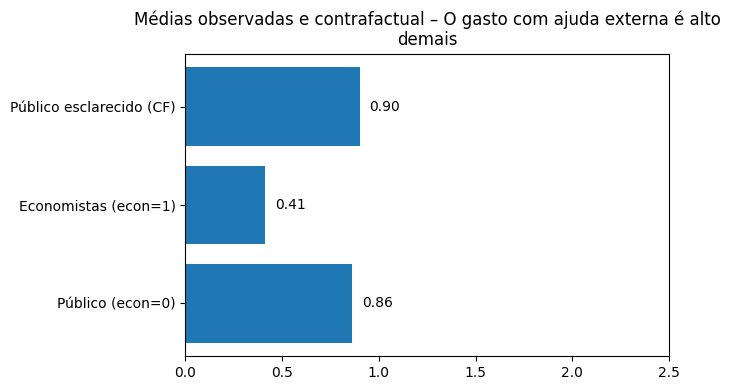
\includegraphics[width=0.8\textwidth]{Textuais/analise/imagens/gasto_ajuda_externa.png}
\notafig
\label{fig:ajuda}
\end{figure}

\begin{figure}[htbp]
\centering
\caption{Médias de concordância com a afirmação ``Os impostos são muito altos'' para o público geral, o público ``contrafactual'' e os economistas.}
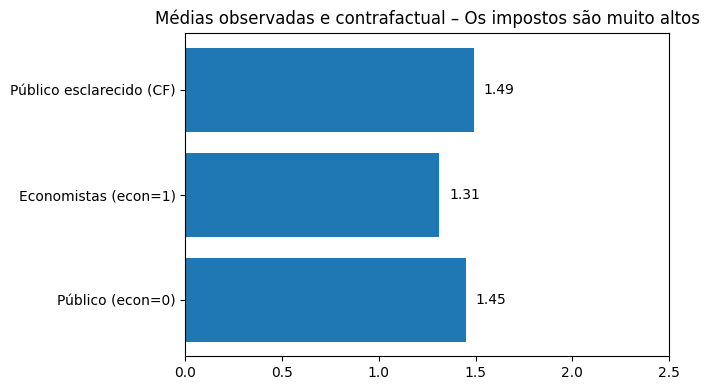
\includegraphics[width=0.8\textwidth]{Textuais/analise/imagens/impostos_muito_altos.png}
\notafig
\label{fig:impostos}
\end{figure}

De forma resumida, a análise integrada dos modelos logit estimados permite destacar os seguintes pontos centrais (ver \autoref{tab:achados}): 

\begin{enumerate}[label=\alph*)]

    \item \textbf{Vieses generalizados}: na \textit{maioria} das 52 questões analisadas, identificam-se diferenças sistemáticas entre grupos de respondentes, compatíveis com vieses descritos na literatura (antimercado, antiestrangeiro, antitrabalho, pessimista) \cite{The_Myth_of_the_Rational_Voter}.

    \item \textbf{Influência dominante da ideologia}: em grande parte das variáveis dependentes (DVs), o coeficiente associado ao espectro ideológico foi estatisticamente significativo (com frequência \(p<0{,}01\)), ao passo que o coeficiente de formação em Economia (indicador de conhecimento especializado) alcançou significância em um subconjunto menor de DVs. Ademais, a magnitude típica dos efeitos ideológicos superou a dos efeitos de conhecimento: na \textit{escala de log-odds} dos modelos ordenados, \(|\beta_{\text{ideologia}}|\) concentrou-se tipicamente entre 0{,}5 e 0{,}9, enquanto \(|\beta_{\text{econ}}|\) se situou em torno de 0{,}2–0{,}7 nos casos significativos. Em termos substantivos, posicionar-se à direita (versus à esquerda) alterou substancialmente as probabilidades de concordar com proposições como “a dívida pública é grande demais” (ver \autoref{fig:deficit}) ou “as políticas de cotas são excessivas”, ao passo que possuir formação em Economia (versus ser leigo) produziu efeito menor, embora não desprezível.
    
    \item \textbf{Consensos técnicos versus divisões valorativas}: alguns itens revelam consenso amplo entre público e economistas (ausência de viés), sobretudo em princípios econômicos tradicionais; já em temas socioeconômicos carregados de valores, observam-se clivagens acentuadas por ideologia, independentemente de conhecimento.
    
    \item \textbf{Conhecimento como “freio” pontual}: a formação econômica mostrou impacto notável em corrigir percepções factuais equivocadas em certos itens — isto é, quando a desinformação objetiva era o motor dominante — aproximando as respostas de economistas e de leigos “contrafactual”, ainda que sem alterar preferências guiadas por valores.
    
    \item \textbf{Robustez dos padrões}: os resultados mantêm-se consistentes com a inclusão de controles demográficos e socioeconômicos, sugerindo que os efeitos de ideologia e conhecimento não decorrem de fatores de confusão evidentes.
\end{enumerate}

\section{O público contrafactual como régua entre ideologia e informação} 

Para quantificar separadamente os efeitos da ideologia e do conhecimento, definiu-se o chamado \textit{público contrafactual} como um experimento contrafactual: trata-se da opinião média prevista caso os respondentes leigos tivessem nível de informação equivalente ao dos economistas, mantendo-se seus demais atributos constantes (em particular, conserva-se a distribuição original de orientações ideológicas). Em outras palavras, o público contrafactual simula qual seria a percepção popular na ausência de déficits de conhecimento técnico. Como era de se esperar, nas figuras observamos que esse grupo hipotético tende a ocupar uma posição intermediária entre o público geral e os economistas. 

Essa posição serve como uma régua de comparação que permite discernir, em cada questão, o peso relativo da ideologia (diferença entre as opiniões do público contrafactual e dos economistas) em contraste com o peso da informação (diferença entre o público geral e o contrafactual). Se a introdução de conhecimento técnico (passando do público geral ao contrafactual) pouco altera a opinião média, conclui-se que o fator ideológico domina naquela questão; por outro lado, se o público contrafactual praticamente converge com os economistas, infere-se que o gap original decorria majoritariamente de desinformação. 

A seguir, organizam-se os achados por blocos temáticos, discute-se o peso relativo de ideologia e informação e, por fim, avaliam-se robustez, limitações e implicações à luz das hipóteses do estudo.

\begin{quadro}[!htb]\centering\footnotesize
\caption{Principais achados dos resultados empíricos}\label{tab:achados}
\begin{tabular}{p{5.5cm} p{9.5cm}}
\toprule
\textbf{Achado-chave} & \textbf{Evidências selecionadas} \\
\midrule
\textbf{Ideologia como filtro dominante} & Coeficientes ideológicos significativos na \textit{maioria} das 37 regressões (em muitos casos com \(p<0{,}01\)). Efeito típico: \(|\beta_{\text{ideologia}}|\approx0{,}5\text{–}0{,}9\) (log-odds), superando o impacto do conhecimento. P.\,ex., respondentes à direita tenderam mais a ver a dívida pública como “grande demais” e a rejeitar maior intervenção estatal; à esquerda verificou-se o padrão inverso. \\
\textbf{Conhecimento técnico corrige desinformação} & Coeficientes de “formação em Economia” significativos em cerca de um terço dos modelos, geralmente \(|\beta_{\text{econ}}|\approx0{,}2\text{–}0{,}7\). P.\,ex., economistas (controlada a ideologia) discordaram em proporção maior de “gasta-se muito com ajuda externa” (\autoref{fig:ajuda}), ajustando uma crença popular que superestima essa rubrica; de modo análogo, mostraram menor alarme em relação ao déficit público (\autoref{fig:deficit}), em linha com critérios técnicos de sustentabilidade fiscal \cite{The_Myth_of_the_Rational_Voter}. \\
\textbf{Consenso em bases econômicas} & Diversas questões de economia básica e reformas estruturais apresentaram concordância ampla entre grupos. P.\,ex., “A reforma tributária é necessária” obteve concordância elevada entre leigos e economistas (médias de resposta \(\approx1{,}81\) e \(\approx1{,}94\), respectivamente), sem clivagem ideológica robusta. Em contrapartida, \textit{reforma previdenciária} e \textit{trabalhista} exibem apoio majoritário, porém com gradiente ideológico significativo (direita apoia mais). \\
\textbf{Clivagens socioideológicas acentuadas} & Em itens distributivos e de avaliação do setor privado — p.ex., “empresas lucram demais”, “salários de altos executivos são excessivos”, “ações afirmativas dão vantagens demais” — observa-se clivagem marcada: o público leigo mostrou-se relativamente mais crítico que economistas, e as respostas polarizaram por ideologia. A interpretação é compatível com o papel das narrativas político-emocionais na formação de crenças \cite{westen2007political}. \\
\textbf{Viés pessimista e outras tendências} & Identifica-se um viés pessimista relevante: parcela expressiva dos eleitores avaliou a situação (atual e futura) de forma mais negativa do que economistas, notadamente em desigualdade e renda real ao longo do tempo; padrões transversais por sexo e idade também emergem (homens mais céticos quanto à regulação e menos críticos a salários executivos; faixas de 46–55 e 66+ mais sensíveis a temas como juros e corrupção). \\
\bottomrule
\end{tabular}
\end{quadro}

\section{Resultados por Bloco Temático de Variáveis Dependentes}
Os padrões observados permitem agrupar as questões em blocos temáticos conforme suas dinâmicas substantivas comuns. Em vez de examinar cada pergunta isoladamente, a seguir sintetizamos os resultados por conjunto de itens relacionados, destacando exemplos representativos e conectando-os às hipóteses teóricas relevantes.

\subsection{Consenso em Políticas Econômicas Estruturais}
Em diversas perguntas sobre princípios de economia e reformas estruturais observou-se convergência ampla nas opiniões dos segmentos analisados. Em particular, no item ``\textit{A reforma tributária é necessária}'' verificou-se concordância praticamente unânime entre respondentes com e sem formação em Economia (médias de resposta, respectivamente, $\approx1{,}94$ e $\approx1{,}81$, em escala Likert de 0 sendo ``discordo totalmente'' a 2 sendo ``concordo totalmente''), sem diferenças ideológicas ou educacionais robustas. Por outro lado, em ``\textit{A reforma da previdência é necessária}'' e ``\textit{A reforma trabalhista é necessária}'', embora o apoio seja majoritário, persiste o gradiente ideológico estatisticamente significativo (maior apoio entre respondentes à direita). Em síntese, identifica-se um núcleo de consenso real em matérias estruturais (p.\,ex., a necessidade de revisar o arranjo tributário), ao passo que, em outras reformas, o apoio amplo convive com clivagens ideológicas previsíveis. Essa configuração é compatível com a distinção de \cite{sowell2007conflict} entre ``visões'' de mundo: quando o diagnóstico técnico é menos controverso moralmente, mesmo agentes com informação limitada tendem a alinhar suas crenças ao consenso pericial.

\subsection{Divergências Ideológicas em Questões Socioeconômicas}
Em contraste com os consensos acima, um segundo bloco reúne itens com conotação ideológica/distributiva mais saliente, em que despontam divergências marcantes entre grupos. Entram aqui enunciados como ``\textit{As empresas têm lucros demasiadamente altos}'', ``\textit{Os salários dos altos executivos são excessivos}'', ``\textit{As ações afirmativas dão vantagens demais para minorias}'', ``\textit{Ter mais mulheres na força de trabalho é algo positivo}'' e “\textit{os impostos são muito altos}”, que exibe gradiente ideológico nítido (\autoref{fig:impostos}). Os resultados indicam que o público leigo se mostrou relativamente mais crítico que os economistas em relação a lucro privado e remuneração executiva, com clivagem ideológica pronunciada (maior concordância à esquerda e menor à direita). 

Tal padrão é compatível com o viés antimercado discutido por \citeonline{The_Myth_of_the_Rational_Voter}, segundo o qual eleitores tendem a superestimar efeitos negativos atribuídos ao mercado e a favorecer correções estatais. A leitura também dialoga com a tipologia de visões proposta por \citeonline{sowell2007conflict}: a ``visão constrangida'' tende a reconhecer trade-offs e a valorizar mecanismos de mercado, ao passo que a ``visão não constrangida'' mostra maior propensão a soluções igualitaristas. Ademais, como argumenta \citeonline{westen2007political}, identidades e afetos partidários modulam a recepção de evidências, de modo que direita e esquerda filtram o mesmo fato por lentes normativas distintas. Em termos empíricos, a variável de \textit{espectro ideológico} emerge significativa na maioria desses itens polarizadores, configurando um espelhamento ideológico robusto: esquerda associa problemas a ``falhas de mercado'' e demanda regulação/redistribuição; direita associa problemas a ``falhas de governo'' e demanda restrição a gastos/intervenção.

\subsection{Questões de Viés Informacional e Correções pelo Conhecimento}
Um terceiro padrão envolve itens nos quais a assimetria informacional aparece como mecanismo central de divergência entre opinião popular e leitura técnica. Nesses casos, controlada a ideologia, a formação em Economia associa-se a respostas significativamente distintas do público leigo, sugerindo que a variação decorre de diferenças de informação.

O exemplo mais claro é ``\textit{O gasto com ajuda externa é alto demais}''. Aqui, identificou-se efeito ideológico positivo (respondentes mais à direita concordam mais) e um efeito corretivo de formação (coeficiente negativo significativo para a dummy de Economia): economistas, independentemente de sua orientação política, tendem a discordar do enunciado, coerentes com o fato de que tal rubrica representa parcela diminuta do orçamento. Em outras palavras, a informação especializada reduz uma percepção equivocada que atravessa o espectro político. Esse ajuste é visível no contraste entre as três barras de \autoref{fig:ajuda}.

Padrão análogo surge em ``\textit{O déficit federal é grande demais}'': o coeficiente ideológico é positivo e altamente significativo (maior preocupação à direita), enquanto a dummy de formação em Economia é negativa e significativa, indicando menor alarmismo entre os tecnicamente informados (médias $\approx1{,}51$ no público leigo versus $\approx1{,}12$ entre economistas). Essa combinação sustenta a afirmação anterior acerca de viés \textit{pessimista} do eleitor e de que o conhecimento atua como \textbf{freio epistêmico}, atenuando leituras alarmistas infundadas. O padrão de menor alarmismo técnico aparece em \autoref{fig:deficit}.

Há, ainda, casos em que o público tende a \textit{subestimar} problemas estruturais pouco salientes intuitivamente. Em ``\textit{A produtividade aumenta devagar demais}'' e em ``\textit{Empresas estão enviando funcionários ao exterior}'', a formação em Economia associa-se a \textbf{maior preocupação} com entraves de produtividade e offshoring (efeitos positivos e significativos), sugerindo que a informação técnica desloca a atenção para fricções menos visíveis no debate cotidiano. Em suma, quando a questão envolve fatos pouco intuitivos, o conhecimento especializado aproxima as respostas do \textit{consenso técnico}, corroborando a hipótese de que a instrução econômica reduz a propensão a vieses informacionais, sem, contudo, eliminar divergências motivadas por valores.

\subsection{Outros Padrões Transversais e Surpresas}
Para além dos agrupamentos principais, identificaram-se padrões transversais e alguns resultados inesperados. Em primeiro lugar, destaca-se um gradiente geracional moderado: respondentes mais jovens (até aproximadamente 25 anos) tenderam a atribuir menor gravidade a passivos de longo prazo (v.g., dívida pública e sustentabilidade previdenciária), ao passo que indivíduos de meia-idade (aproximadamente 35--55 anos) revelaram maior pessimismo quanto ao futuro econômico e à evolução da renda. Tal diferença se refletiu em efeitos de idade estatisticamente significativos em itens específicos (ver \autoref{apendice:tabela_sintese}), nos quais participantes acima de 45 anos demonstraram preocupações superiores com perda de postos de trabalho e endividamento do Estado, enquanto os mais jovens mostraram-se relativamente mais otimistas ou indiferentes. Embora menos pronunciados que os efeitos de ideologia, esses padrões são consistentes com a hipótese de que a experiência histórica (p.ex., vivências de inflação elevada e recessões) molda expectativas econômicas.

Em segundo lugar, observaram-se diferenças sistemáticas por sexo. Em média, homens mostraram menor propensão a apoiar intervenções redistributivas e maior alinhamento a perspectivas pró-mercado em itens específicos. Exemplificativamente, homens discordaram mais da afirmação ``\textit{executivos ganham demais}'' e concordaram mais com ``\textit{o governo regulamenta muito os negócios}''; adicionalmente, foram relativamente menos favoráveis ao enunciado ``\textit{ter mais mulheres na força de trabalho é positivo}''. Esses achados sugerem que parte das avaliações normativas sobre regulação, remuneração e papéis de gênero varia por sexo, possivelmente refletindo heterogeneidades de valores culturais e posições socioeconômicas médias.

Por fim, quanto às perplexidades, dois casos merecem registro. Primeiro, no item ``\textit{o gasto com ajuda externa é alto demais}'', detectou-se um duplo mecanismo: (i) efeito ideológico \textit{positivo} e estatisticamente significativo (maior concordância entre respondentes à direita) e (ii) efeito \textit{corretivo} da formação em Economia (coeficiente negativo significativo), o que indica que conhecimento especializado atenua uma percepção superestimada disseminada no público. Segundo, no item referente à ``\textit{fuga de talentos}'' (empresas enviando profissionais ao exterior), economistas demonstraram maior preocupação do que leigos, padrão compatível com uma assimetria informacional em que o grupo tecnicamente informado detecta um problema estrutural pouco saliente para o público geral. Esses episódios, embora minoritários, ilustram que nem todas as divergências ou convergências se explicam por um único tipo de viés: há casos de \textit{desinformação difusa} (corrigida pelo conhecimento) e casos em que especialistas antecipam riscos latentes ausentes da percepção pública. Em ambos, ressalta-se o papel do conhecimento como mecanismo de ajuste das percepções a parâmetros factuais.

\section{Ideologia vs. Informação: Qual Fator Pesa Mais}

A questão central consiste em determinar, frente a discrepâncias entre a opinião pública e o consenso técnico, a contribuição relativa de vieses ideológicos em contraste com déficits informacionais. A estratégia empírica adotada estimou, de modo comparável entre itens, modelos com variáveis de ideologia (espectro político) e de conhecimento (formação em Economia), sob controle demográfico e socioeconômico. A geometria típica das três barras (Geral–Contrafactual–Economistas) nas \autoref{fig:deficit}–\autoref{fig:impostos} ilustra essa hierarquia: a ideologia desloca o nível médio, enquanto o conhecimento encurta a distância quando o item é informacional.

Os resultados são inequívocos. Em quase todas as 52 variáveis dependentes, o alinhamento ideológico apresentou efeito estatisticamente significativo e substantivo, ao passo que a formação em Economia exibiu impactos \textit{pontuais} e de menor magnitude média (ainda que relevantes nos itens informacionais). Em termos agregados, os valores absolutos de $\beta_{\text{ideologia}}$ situaram-se tipicamente em 0{,}5--0{,}9, superando os de $\beta_{\text{econ}}$ (em torno de 0{,}2--0{,}7 nos casos significativos). Substantivamente, a identificação com a direita (versus esquerda) ampliou a probabilidade de concordância com proposições como ``\textit{o déficit é grande demais}'' ou ``\textit{o governo deve intervir menos}'', enquanto a formação econômica produziu ajustes mais modestos nessas probabilidades.

Em síntese, no impacto imediato sobre crenças econômicas, a filiação ideológica opera como filtro cognitivo mais potente e consistente que a instrução técnica --- dinâmica congruente com o viés de confirmação e a cognição cultural documentados pela literatura \cite{kahneman2011thinking, kahan2012polarization}. Por outro lado, o conhecimento econômico funciona como \textit{limite epistêmico} que corrige erros factuais e aproxima respostas do \textit{consenso técnico} quando a questão envolve conteúdo pouco intuitivo (v.g., composição orçamentária, dinâmica da produtividade), em linha com a tese de que os eleitores manifestam vieses sistemáticos \cite{The_Myth_of_the_Rational_Voter}. Em matérias de consenso técnico robusto (p.ex., a necessidade de controlar a inflação ou benefícios do comércio), tampouco se observaram clivagens relevantes, reforçando que, ausente carga valorativa forte, mesmo agentes com informação limitada convergem.

Do ponto de vista aplicado, decorre que a ``\textit{verdade técnica}'', isoladamente, mostra-se insuficiente para moldar crenças políticas quando estas se ancoram em identidades e valores \cite{westen2007political}. Políticas públicas baseadas em evidências demandam, simultaneamente, (i) educação econômica para reduzir erros factuais e (ii) \textit{molduras comunicacionais} (frames) que dialoguem com repertórios normativos distintos, evitando dissonâncias identitárias que levam à rejeição de evidências. Assim, mais que opor conhecimento e ideologia, impõe-se reconciliá-los: integrar fatos verificáveis a narrativas legitimadas pelos grupos destinatários, de modo a reduzir o descompasso entre consenso técnico e crença popular.

\section{Robustez dos Resultados e Limitações do Estudo}
\label{sec:limitacao_robustez}
Do ponto de vista metodológico, procederam-se a checagens destinadas a assegurar a robustez das inferências e a explicitar limitações do desenho empírico. Em primeiro lugar, os modelos foram estimados sob uma especificação uniforme (mesmo conjunto de covariáveis) para todas as 52 DVs. Essa estratégia favorece a comparabilidade direta dos coeficientes entre itens e reduz o risco de viés por variação de especificação. A Tabela-Síntese Mestra (Apêndice \autoref{apendice:tabela_sintese}) consolida os coeficientes nessa escala comum, facilitando a identificação de regularidades de sinal e significância.

No que concerne ao ajuste, empregou-se o modelo logit ordenado com tentativa principal por L-BFGS e fallback programado para BFGS e Powell. Procedeu-se a uma verificação heurística da plausibilidade dos limiares por meio da ordenação dos cutpoints; quando essa ordenação se mostrou inadequada ou quando houve falha de convergência, o item foi assinalado como não estimável ou não estável na Tabela-Síntese (ver \autoref{apendice:tabela_sintese}). No que tange à multicolinearidade, não foram calculadas medidas formais (por exemplo, VIF); a mitigação adotada consistiu na remoção de colunas constantes ou raras e no acompanhamento da estabilidade de sinais e incertezas. Registre-se, ainda, que não foi implementado o teste formal da suposição de chances proporcionais por item (por exemplo, Brant), e os erros-padrão reportados são os do estimador. 

Essas escolhas foram realizadas a fim de privilegiar a parcimônia, comparabilidade e congruência: evitam ampliar graus de liberdade do pesquisador com baterias de testes item a item, mantêm uma régua comum entre especificações e concentram a validação no que é condição de admissibilidade do modelo (ordem dos limiares) e em critérios práticos de estabilidade numérica. Em amostras moderadas com múltiplas DVs, testes de Brant por item aumentam a multiplicidade sem ganho proporcional de inferência; O VIF é de interpretação pouco informativa, com muitas dummies e colinearidades estruturais conhecidas, cujo remédio efetivo é o desenho do modelo (remoção de colunas degeneradas) e a verificação da estabilidade dos sinais ao longo dos 52 itens; Como cada regressão usa uma única DV por respondente, não há estrutura de cluster adicional a modelar no nível do item, tornando adequados os erros-padrão do estimador alinhados à especificação adotada.

Realizou-se, adicionalmente, o cálculo de um contrafactual para o subgrupo de economistas: predições foram obtidas \textit{como se} a variável de formação em Economia assumisse o valor zero para os respondentes com \(\mathrm{econ}=1\). Esse procedimento fornece a ``média contrafactual'' reportada na Tabela-Síntese e permite comparar a distância entre o grupo tecnicamente formado e seu cenário sem formação específica, mantendo constantes as demais covariáveis.

Algumas limitações estatísticas merecem destaque. Em itens com alto consenso na amostra (\textit{quase-separação}), a estimação torna-se instável e os erros-padrão inflacionam, o que justifica a rotulagem de modelos como não estimáveis/instáveis. Ademais, certos subgrupos, notadamente respondentes com formação em Economia, são reduzidos, o que limita o poder estatístico para detectar efeitos da variável \(\mathrm{econ}\) em todas as DVs. Ainda assim, quando presente, o efeito de formação mostrou-se suficientemente pronunciado em itens informacionais para emergir do ruído.

No plano amostral, a coleta por \textit{bola de neve} online visou maximizar a heterogeneidade ideológica e educacional para teste sob severidade, não assegurar representatividade populacional estrita. Consequentemente, níveis absolutos de concordância não devem ser extrapolados mecanicamente ao eleitorado brasileiro; o foco recai sobre padrões condicionais (diferenças entre grupos sob controles), que podem ser informativos de mecanismos cognitivos gerais. 

Por fim, a interpretação é não causal. Apesar de controles observáveis, não se pode inferir que a formação em Economia cause mudanças de opinião de modo exógeno — processos de auto-seleção podem estar presentes; de modo análogo, diferenças ideológicas podem refletir determinantes culturais de longo prazo. Os achados devem, assim, ser entendidos como associações condicionais válidas no escopo do desenho e dos pressupostos modelados \cite{hausman2008}. Nesses termos, constituem evidência compatível com teorias de vieses, mas não prova irrefutável — corroboração sujeita a refutação mediante novos dados ou estratégias inferenciais alternativas \cite{popperlogic}.

\subsection{Por que usar o mesmo modelo para todas as DVs}\label{sec:modelo-unico}
Aplicamos o mesmo modelo logit ordenado, com as mesmas variáveis explicativas e controles, nas 52 regressões estimadas. Longe de ser uma simplificação ad hoc, essa decisão atende a quatro razões de método e comunicação científica:

\begin{enumerate}[label=\roman*)]
\item \textbf{Teste severo e comparabilidade popperiana.} Submeter cada hipótese de viés ao mesmo escrutínio reduz os graus de liberdade do pesquisador, desincentiva \emph{data mining} e fortalece a lógica de falseabilidade: se um efeito só aparece em especificações “sob medida”, sua robustez é duvidosa; se reaparece em itens distintos dentro do mesmo arcabouço, ganha força inferencial.

\item \textbf{Princípios-ponte e inteligibilidade teórica.} Uma especificação única funciona como uma “régua comum”: os coeficientes de ideologia e formação econômica tornam-se diretamente comparáveis entre DVs, dando conteúdo empírico uniforme aos constructos de “viés ideológico” e “efeito de conhecimento”, em linha com a busca de congruência teórico–empírica \cite{stigum2003}. Essa escolha dialoga com os princípios-ponte descritos na \autoref{sec:escopo-inferencial} e com as decisões de comparabilidade na \autoref{sec:pressupostos-inferencia}.

\item \textbf{Coerência com visões e efeito de formação.} Se visões de mundo e treinamento econômico permeiam múltiplas crenças, um modelo unificado é o desenho natural para capturar o fio condutor latente. Mantendo a estrutura fixa, observamos a onipresença do efeito ideológico e identificamos onde o conhecimento realmente desloca crenças \cite{sowell2007conflict,newman2020ideia}. 

\item \textbf{Comunicabilidade e síntese.} A \textbf{Tabela-Síntese Mestra} (\autoref{apendice:tabela_sintese}) só é possível porque os coeficientes “vivem” na mesma escala; isso permite contar significâncias, comparar magnitudes e contar uma narrativa unificada sobre quando a verdade técnica converge/diverge da opinião popular.
\end{enumerate}

\section{Síntese dos Resultados Frente aos Objetivos e Hipóteses}\label{sec:sintese-resultados}

Em consonância com a \autoref{sec:objetivo-geral} e com os objetivos específicos listados na \autoref{sec:objetivos-especificos}, de \autoref{obj:a} até \autoref{obj:e}, os achados permitem uma avaliação integrada do grau em que os objetivos foram atendidos e das hipóteses (H1–H7) à luz dos dados. Os dados no \autoref{apendice:tabela_sintese} evidenciam, de forma comparativa, quais vieses e clivagens emergem de modo consistente. A seguir, confronta-se cada hipótese com as evidências empíricas e indica-se sua conexão com os objetivos.

\textbf{H1 (Vieses populares sistemáticos)} — \textit{Eleitores brasileiros apresentam vieses cognitivos sistemáticos que distorcem sua percepção econômica}. Os resultados sustentam a hipótese. Observa-se, em múltiplos itens, um padrão de respostas compatível com os vieses \emph{antimercado}, \emph{antiestrangeiro}, \emph{antitrabalho} e \emph{pessimista}, conforme a tipologia proposta na literatura \cite{The_Myth_of_the_Rational_Voter}. A presença de diferenças regulares entre o público leigo e os respondentes com formação econômica, bem como entre espectros ideológicos, indica que tais desvios não são aleatórios, mas estruturados. Conclui-se, portanto, que H1 foi corroborada, atendendo diretamente aos objetivos \autoref{obj:c} (mapear presença/frequência) e \autoref{obj:d} (discrepâncias vs.\ consenso técnico).

\textbf{H2 (Conhecimento reduz vieses)} — \textit{O conhecimento econômico reduz a probabilidade de manifestação de vieses cognitivos}. A evidência é parcialmente favorável. A variável de formação em Economia apresenta significância em cerca de um terço dos modelos, com associações alinhadas ao consenso técnico em itens de natureza predominantemente informacional (p.\,ex., percepção sobre gasto externo e \emph{alarmismo} com a dívida). Isso é congruente com o papel de heurísticas e vieses na formação de crenças e com a atenuação propiciada por conhecimento específico \cite{kahneman2011thinking,Judgment_under_Uncertainty, The_Myth_of_the_Rational_Voter}. Por outro lado, em temas carregados de valores, o efeito do conhecimento mostrou-se limitado. Assim, H2 é corroborada com ressalvas, contribuindo para os objetivos \autoref{obj:d} (determinantes das discrepâncias) e \autoref{obj:e} (associações com variáveis educacionais).

\textbf{H3 (Viés antimercado e políticas intervencionistas)} — \textit{O viés antimercado está associado ao apoio a políticas intervencionistas}. As estimativas indicam que respondentes com posições críticas em relação aos lucros e à competição tendem a apoiar maior intervenção estatal, controle e regulação, ao passo que perfis pró-mercado rejeitam tais proposições, em linha com Sowell (\citeyear{sowell2000basic,sowell2007conflict,sowell2004applied}). H3 é, portanto, corroborada, alinhada aos objetivos \autoref{obj:d} (padrões de discrepância e seus determinantes) e \autoref{obj:e} (associações com covariáveis).

\textbf{H4 (Viés antiestrangeiro e protecionismo)} — \textit{O viés antiestrangeiro está associado ao apoio a restrições comerciais e migratórias}. Registra-se associação entre maior predisposição protecionista e visões céticas quanto à concorrência externa, enquanto posições favoráveis à abertura apresentam o padrão oposto, compatível com os benefícios de especialização e vantagem comparativa discutidos na literatura \cite{bhagwati2003free, The_Myth_of_the_Rational_Voter}. H4 é corroborada; a conexão com os objetivos \autoref{obj:d} e \autoref{obj:e} é direta (determinantes e associações). Note-se, contudo, que a questão específica sobre imigração não produziu clivagens estatisticamente significativas, o que pode refletir o contexto brasileiro recente.

\textbf{H5 (Viés antitrabalho e políticas de emprego direto)} — \textit{O viés antitrabalho está associado ao apoio a políticas que priorizam a criação direta de empregos em detrimento da eficiência}. As evidências são mistas. Identifica-se ceticismo quanto à qualidade de novos postos e menor ênfase leiga em produtividade; porém, a proposição de que a automação “prejudica” o mercado de trabalho foi majoritariamente rejeitada, o que não coaduna com um ludismo generalizado. A literatura alerta que a supervalorização do emprego \emph{per se} pode colidir com os ganhos de eficiência de longo prazo \cite{landsburg2012armchair,sowell2007conflict}. Assim, H5 recebe apoio parcial, contribuindo para os objetivos \autoref{obj:d} e \autoref{obj:e}.

\textbf{H6 (Viés pessimista)} — \textit{O viés pessimista leva a avaliações mais negativas do que os dados indicam}. A hipótese é amplamente confirmada: em itens sobre trajetória de desigualdade, padrão de vida e rendas relativas a preços, nota-se uma avaliação mais negativa no público leigo, enquanto os respondentes com formação econômica mostram um menor pessimismo médio. O padrão está em consonância com evidências de desalinhamento entre percepções e séries históricas \cite{easterbrook2004progress, ridleyotimista}. H6 é, portanto, corroborada, atendendo aos objetivos \autoref{obj:c} (presença/frequência) e \autoref{obj:d} (discrepâncias frente a dados/consenso).

\textbf{H7 (Influência da ideologia sobre evidências)} — \textit{A filiação ideológica influencia a aceitação das evidências econômicas}. A variável ideologia surge como preditor substantivo na quase totalidade das DVs, com efeitos frequentemente superiores aos de conhecimento, indicando filtragem de informações por identidades e valores, conforme a teoria da cognição cultural \cite{kahan2012polarization}. Evidências recentes sobre crenças em desinformação também apontam para uma forte mediação ideológica \cite{rossini2023explaining}. H7 recebe forte suporte, contribuindo centralmente para o objetivo \autoref{obj:e} (associações) e, por consequência, para \autoref{obj:d} (determinantes).

\subsection{Síntese frente aos objetivos.}
Mensuraram-se vieses de julgamento em percepções econômicas \autoref{obj:c}, mapearam-se discrepâncias entre a opinião popular e o consenso técnico e seus determinantes \autoref{obj:d}, e avaliaram-se associações com variáveis sociocognitivas — com destaque para a ideologia e o conhecimento \autoref{obj:e}. Esses resultados se inserem no escopo da \autoref{sec:objetivo-geral} e são viabilizados pelo instrumento descrito no Capítulo de métodos, em atendimento ao \autoref{obj:b}; o \autoref{obj:a} é suportado tanto pela revisão teórica quanto pela validação empírica dos constructos. No conjunto, delineia-se o seguinte quadro: a ideologia atua como filtro dominante e persistente, ao passo que o conhecimento opera como freio epistêmico pontual — eficaz para corrigir erros factuais, mas menos influente em clivagens valorativas. Tais conclusões são consistentes com a literatura de economia política comportamental e informam implicações para a comunicação de políticas públicas ancoradas simultaneamente em evidência e em molduras normativas reconhecíveis pelos diferentes públicos \cite{kahneman2011thinking, kahan2012polarization, Systematically_Biased_Beliefs_about_Economics}.

% \include{Textuais/conclusão}

% -----------------------------------------------------------------
% ELEMENTOS PÓS-TEXTUAIS
% -----------------------------------------------------------------
\postextual

% Você pode comentar os elementos que não deseja em seu trabalho; 

% Referências bibliográficas

%Notar que os autores continuam sendo transpostos em maiúsculas, como preconiza a ABNT NBR 6023:2002. 
%Se, no entanto, não desejar seguir esta regra,
%crie um novo arquivo .bst (por exemplo, novoestilo.bst)a partir do estilo
%usado (abntex2-cite-alf ou abntex2-cite-num) e retire todas as expressões
%"u" change.case$, lembrando-se de indicar o novo arquivo como estilo, por exemplo, 
%\bibliographystyle{novoestilo}, e colocar o arquivo criado na mesma
%pasta em que está compilando o documento.

% Arquivo alterado para citação (Autor, Ano) ao invés de (AUTOR, Ano) conforme ABNT NBR 10520:2023
\bibliographystyle{abntex2-alf_revNBR2023.bst}	

\bibliography{referencias}	% Elemento Obrigatório

% ----------------------------------------------------------
% Glossário
% ----------------------------------------------------------

%Consulte o manual da classe abntex2 para orientações sobre o glossário.

%\glossary




% ----------------------------------------------------------
% Glossário (Formatado Manualmente)
% ----------------------------------------------------------

\chapter*{GLOSSÁRIO}
\addcontentsline{toc}{chapter}{GLOSSÁRIO}

{ \setlength{\parindent}{0pt} % ambiente sem indentação

\textbf{Amostragem não probabilística}: Procedimento de seleção de respondentes sem sorteio aleatório; adequado a testes de hipótese sob severidade, mas com generalização populacional limitada. 

\textbf{Análise contrafactual}: Estimativa de como seria a resposta de um indivíduo sob uma condição hipotética (mantidas as demais características constantes), usando parâmetros de um modelo ajustado.

\textbf{Bola de neve (amostragem)}: Técnica de recrutamento em que participantes indicam novos respondentes, útil para ampliar o alcance da coleta.

\textbf{Coeficiente $\boldsymbol\beta$}: Parâmetro de regressão que quantifica a associação entre uma covariável e a probabilidade (ou categoria) de resposta prevista pelo modelo.

\textbf{Dummy (variável indicadora)}: Variável binária ($0/1$) que representa a presença/ausência de uma característica (por ex., formação em Economia), incluída como regressora no modelo.

\textbf{Escala Likert}: Escala ordinal de resposta (ex.: 3 a 5 pontos) usada para medir concordância/discordância com afirmações.

\textbf{Erros-padrão robustos}: Estimativas de incerteza ajustadas para heteroscedasticidade, tornando a inferência menos sensível a violações de variância constante.

\textbf{Hipótese de chances proporcionais (paralelismo)}: Suposição do logit ordenado de que o efeito das covariáveis é constante entre limiares/categorias; quando plausível, facilita comparabilidade entre itens.

\textbf{Instrumento de pesquisa (questionário)}: Conjunto estruturado de questões aplicado digitalmente, revisado por especialistas e pré-testado para clareza, tempo de resposta e validade de conteúdo.

\textbf{Limiares ($\boldsymbol{\tau_j}$)}: Parâmetros do logit ordenado que definem as fronteiras entre categorias da variável dependente.

\textbf{Logit (modelo)}: Regressão para variáveis dependentes binárias, que modela a probabilidade de um evento via função logística.

\textbf{Logit ordenado}: Extensão do logit para variáveis dependentes ordinais (ex.: Likert), com estrutura de limiares e, usualmente, hipótese de chances proporcionais.

\textbf{Princípios-ponte}: Conjunto de regras que conecta teoria e dados no desenho empírico (operacionalização, codificação/direção esperada e sinal teórico dos efeitos).

\textbf{Público esclarecido (contrafactual)}: Referência simulada que prevê como economistas responderiam “como se fossem leigos” (sem formação econômica), mantendo constantes as demais variáveis — usada para isolar o papel do conhecimento técnico.

\textbf{Racionalidade limitada}: Ideia de que decisões são tomadas sob informação imperfeita e capacidade cognitiva restrita; no contexto político, ajuda a explicar crenças persistentes e vieses.

\textbf{Validade externa}: Alcance da generalização dos resultados além da amostra estudada; com amostragem não probabilística, a inferência é positiva/explicativa e não descritiva da população.

\textbf{Vieses cognitivos (quatro vieses)}: Padrões sistemáticos de julgamento identificados na literatura (antimercado, antiestrangeiro, antitrabalho e pessimista) que afetam percepções econômicas e preferências por políticas.

} % fim ambiente sem indentação



				% Elemento Opcional

% ----------------------------------------------------------
% Apêndices
% ----------------------------------------------------------

% ---
% Inicia os apêndices
% ---
\begin{apendicesenv}

% Imprime uma página indicando o início dos apêndices
%\partapendices



% ----------------------------------------------------------
\chapter{Quadro Síntese das Abordagens sobre (I)Racionalidade Humana e Política}
% ----------------------------------------------------------

\label{apendice:quadro_iracionalidade}

\begin{quadro}[htbp]
\caption{Quadro Síntese – (I)Racionalidade Humana e Política: Principais Abordagens}

\begin{longtable}{p{0.15\textwidth} p{0.23\textwidth} p{0.34\textwidth} p{0.20\textwidth}}
\toprule
\textbf{Autor/Obra (Ano)} & \textbf{Tópico/Conceito Central} & \textbf{Principais Contribuições e Evidências} & \textbf{Relação com o TCC} \\
\midrule
\endfirsthead
\multicolumn{4}{c}{\textbf{Quadro – Continuação}} \\
\toprule
\textbf{Autor/Obra (Ano)} & \textbf{Tópico/Conceito Central} & \textbf{Principais Contribuições e Evidências} & \textbf{Relação com o TCC} \\
\midrule
\endhead

Adam Smith (1759; 1776) & Moralidade e racionalidade econômica & Integra interesse próprio e normas morais; reconhece limites do modelo racional estrito. & Critica o homo economicus e destaca a ética na decisão pública. \\
Herbert Simon (1955) & Racionalidade Limitada & Mostra que decisões são feitas com informação e tempo limitados; conceito de “satisficing”. & Base para analisar limites cognitivos em escolhas políticas. \\
Kahneman \& Tversky (1974, 2011) & Heurísticas e Vieses Cognitivos & Demonstram vieses como representatividade e ancoragem, fundamentais para economia comportamental. & Explica previsibilidade dos desvios do eleitor médio. \\
Anthony Downs (1957) & Ignorância Racional & Eleitor não busca informação pois custo supera o benefício do voto. & Fundamenta debate sobre baixa informação e democracia. \\
Bryan Caplan (2007) & Irracionalidade Racional & Eleitores mantêm crenças falsas por motivações emocionais, não apenas ignorância. & Mostra padrões sistemáticos de viés com impacto em políticas. \\
Hayek (1945) & Limitação do conhecimento & Defende dispersão do conhecimento, inviabilizando decisões centralizadas. & Sustenta crítica à ilusão de controle racional em políticas. \\
Bhagwati, Sowell, Bastiat & Viés antimercado e antiestrangeiro & Abordam recorrência de protecionismo, desconfiança do livre comércio e argumentos populares falhos. & Ampliam análise sobre vieses e políticas populistas. \\
Nyhan, Kahan, Sunstein, Rossini et al. & Resistência à revisão de crenças & Mostram que vieses de confirmação e bolhas informacionais dificultam revisão de crenças e promovem polarização. & Explicam a persistência da desinformação política. \\
\bottomrule
\end{longtable}
\end{quadro}

\chapter{Epílogo Metafísico: Entre a Evidência e a Esperança \\ \smallskip \textit{(Reflexão Filosófica para Além do Empírico)}}

\noindent
\textbf{Nota de método.} \textit{A partir deste ponto, movo-me do domínio do empiricamente testável para a esfera da reflexão filosófica e institucional. Como Popper recomendaria, assumo aqui apenas conjecturas abertas ao debate, inspiradas — e não determinadas — pelos achados empíricos deste trabalho.}

\vspace{1em}

A política moderna consagrou na democracia a liberdade das massas como princípio supremo. Mas que liberdade é essa? A de fazer tudo o que se quer, mesmo sem saber por quê? Ou a de resistir ao próprio desejo, quando tudo grita por rendição? Talvez liberdade seja, afinal, a capacidade de fazer não o que se quer, mas o que se deve — mesmo (ou sobretudo) quando não se deseja. E o dever, aqui, não nasce de comando externo, mas da gravidade interna de quem aprendeu a discernir.

A democracia, em sua forma atual, opera como o teatro onde desejos transitam com legitimidade garantida. A cada eleição, reencena-se a soberania do querer sobre o dever, do imediato sobre o necessário, do impulso sobre o juízo. O sistema, tal como está, recompensa quem responde rápido, não quem pensa devagar. E há algo de estrutural nisso: o calendário democrático segue o tempo do relógio — mas a justiça segue o tempo da consciência. Como ensinou Santo Agostinho, “há um tempo exterior, que corre; e há um tempo interior, que pondera”. A política deveria aspirar a este último.

É nesse palco que se manifesta o paradoxo já desvelado por Caplan: mesmo eleitores bem-intencionados erram. Erram não por ignorância ocasional, mas por uma racionalidade limitada, sistematicamente enviesada, que prefere o conforto da ilusão ao rigor da verdade. E se, como advertiu Hayek, o conhecimento social está sempre disperso e fragmentado, todo sistema que aposta na onisciência da vontade coletiva naufraga entre o caos e a tirania.

Assim, quando um eleitor escolhe, não apenas escolhe: julga. E esse juízo, por mais livre que pareça, carrega uma cadeia invisível de valores, memórias, convicções e desejos. A liberdade, portanto, não é um ponto de partida; é o último degrau de uma escada moral. Só é verdadeiramente livre quem sabe por que deve escolher o que escolhe — e está disposto a não querer o que não deve.

Se a liberdade for reduzida à soma dos desejos, o resultado será sempre um sistema vulnerável à manipulação, à irracionalidade e à moral líquida. Não há mercado perfeito de ideias, nem há “engenharia institucional” capaz de garantir, por decreto, que a liberdade coincida com o bem comum. Como Acemoglu e Robinson demonstram, a liberdade nasce no estreito corredor entre o excesso de poder e a ausência de ordem: não é dádiva, mas conquista precária, resultado de uma tensão viva entre Estado e sociedade.

Votar é fácil; escolher bem é difícil. Não basta, portanto, melhorar os eleitores. É preciso repensar as engrenagens do sistema que transforma preferências em leis. Um sistema político que se submete inteiramente às oscilações das paixões populares perde sua capacidade de guardar aquilo que não muda: a justiça, o bem, a verdade. Precisamos, pois, de instituições que operem não apenas no tempo do poder, mas no tempo do juízo. E esse tempo não é democrático nem autoritário — é simplesmente humano.

Talvez o caminho esteja em resgatar uma arquitetura política onde a liberdade não seja apenas protegida, mas formada; onde a decisão coletiva seja amparada por raízes mais fundas que as modas da hora; onde o bem comum não seja o resultado do grito da maioria, mas o fruto do silêncio que pensa. Pois, se algo há — e há — é a necessidade de juízo. Porque o nada, isto é, o puro desejo, não institui ordem. Só o ser — aquilo que permanece, que resiste ao fluxo — pode fundar liberdade duradoura.

Este trabalho não pretende esgotar essas possibilidades. Limita-se a constatar, com base empírica e fundamento teórico, que o problema não está apenas nos votos, mas naquilo que os votos ignoram, no que, como diria Bastiat, “o que se vê e o que não se vê”. É preciso olhar para o que não se vê, analisando as evidências com cuidado. E que, para que a verdade tenha alguma chance, será preciso mais do que pedagogia: será preciso estrutura, limite e tempo.

Há decisões que não cabem em ciclos de quatro anos. Há verdades que não se revelam em sondagens. Há justiças que não se alcançam por aclamação. E há liberdades que só florescem quando já não estamos mais olhando para nós mesmos — mas para o bem que nos excede.

A política, quando é séria, não é desejo. É juízo. E o juízo não se apressa. Espera o tempo certo — o tempo do discernimento — para decidir com liberdade verdadeira. Talvez esse tempo ainda venha. Ou talvez já esteja vindo, silencioso, em meio às ruínas de um mundo que confundiu liberdade com vontade e nos deixou uma moral relativa com a qual lidar. Seja como for, uma coisa é certa: não será a pedagogia que nos salvará, mas a arquitetura moral que soubermos legar — e que quisermos deixar — para as próximas gerações.

Por fim, não pretendo impor juízos, mas apenas propor reflexão. Que o dissenso, longe de nos afastar, seja ocasião de busca conjunta por aquilo que resiste ao tempo e nos chama para além de nós mesmos. Não encerro com respostas definitivas, mas com a confissão do limite: a verdade é como a água pura que tentamos reter entre as mãos — ela escorre por entre os dedos, mas ainda assim refresca, orienta e purifica. Talvez, como intuiu Jung, só possamos nos aproximar do valor mais alto reconhecendo aquilo que, em nosso íntimo, ocupa o lugar supremo, fonte de todo sentido. E se toda busca sincera se inclina, por fim, diante desse Bem maior que nos transcende e nos funda, resta-nos apenas o papel de aprendizes: atentos ao mistério, pacientes com o tempo, humildes diante do real.

\begin{flushright}
\textit{
“Ninguém alcança a verdade senão aquele\
que ousa caminhar entre dúvidas,\
mas não abandona a esperança.\
Pois só na humildade diante do Mistério\
a razão encontra repouso e o coração, paz.”\
— inspirado em Santo Agostinho, Confissões
}
\end{flushright}




\end{apendicesenv}
% ---				% Elemento Opcional

% ----------------------------------------------------------
% Anexos
% ----------------------------------------------------------
%
% ---
% Inicia os anexos
% ---
\begin{anexosenv}

	% Imprime uma página indicando o início dos anexos
	%\partanexos

	% ---
	\chapter{Variáveis de controle analisadas por Caplan}

	\begin{longtable}{|>{\raggedright\arraybackslash}p{4cm}
        |>{\raggedright\arraybackslash}p{8cm}
        |>{\raggedright\arraybackslash}p{4cm}|}
\caption{Variáveis de Controle e Codificação (Caplan, 2002)}
\label{tab:caplan_controls} \\
\hline
\textbf{Variável} & \textbf{Pergunta} & \textbf{Codificação} \\
\hline
\endfirsthead

\hline
\textbf{Variável} & \textbf{Pergunta} & \textbf{Codificação} \\
\hline
\endhead

\hline
\endfoot

\hline
\endlastfoot

\textbf{Econ} & – & 1 se economista, 0 caso contrário \\
\hline
\textbf{Black} & Qual é a sua raça? Branco, negro, asiático ou outra? & 1 se negro, 0 caso contrário \\
\hline
\textbf{Asian} & Idem & 1 se asiático, 0 caso contrário \\
\hline
\textbf{Othrace} & Idem & 1 se outra raça, 0 caso contrário \\
\hline
\textbf{Age} & – & 1996 - ano de nascimento \\
\hline
\textbf{Male} & – & 1 se homem, 0 caso contrário \\
\hline
\textbf{Jobsecurity} & Qual o seu nível de preocupação com a possibilidade de perder o emprego no próximo ano? &
3 = “Nada preocupado”; 2 = “Pouco preocupado”; 1 = “Um pouco preocupado”; 0 = “Muito preocupado” \\
\hline
\textbf{Yourlast5} & Nos últimos 5 anos, a renda da sua família cresceu mais rápido, igual ou mais devagar que o custo de vida? &
2 = “Cresceu”; 1 = “Igual”; 0 = “Caiu” \\
\hline
\textbf{Yournext5} & Nos próximos 5 anos, sua renda crescerá mais rápido, igual ou mais devagar que o custo de vida? &
2 = “Crescerá mais rápido”; 1 = “Igual”; 0 = “Mais devagar” \\
\hline
\textbf{Income} & Qual a renda total anual da sua família (antes dos impostos)? &
1 = Até \$10.000; 2 = \$10.001–\$19.999; 3 = \$20.000–\$24.999; 4 = \$25.000–\$29.999; 5 = \$30.000–\$39.999;
6 = \$40.000–\$49.999; 7 = \$50.000–\$74.999; 8 = \$75.000–\$99.999; 9 = \$100.000 ou mais \\
\hline
\textbf{Dem} & Você se considera democrata? & 1 se sim, 0 caso contrário \\
\hline
\textbf{Rep} & Você se considera republicano? & 1 se sim, 0 caso contrário \\
\hline
\textbf{Indep} & Você se considera independente? & 1 se sim, 0 caso contrário \\
\hline
\textbf{Othparty} & Você pertence a outro partido? & 1 se sim, 0 caso contrário \\
\hline
\textbf{Ideology} & Como você se classifica ideologicamente? &
-2 = “Muito liberal”; -1 = “Liberal”; 0 = “Moderado”; 1 = “Conservador”; 2 = “Muito conservador”; 3 = “Não pensa nesses termos” \\
\hline
\textbf{Othideol} & Dummy para ideologia indefinida & 1 se Ideology = 3, 0 caso contrário \\
\hline
\textbf{Education} & Qual o maior nível de escolaridade que você concluiu? &
1 = Fundamental (1ª–8ª); 2 = Ensino médio incompleto; 3 = Ensino médio completo;
4 = Técnico/profissionalizante; 5 = Superior incompleto; 6 = Superior completo; 7 = Pós-graduação \\
\end{longtable}

\vspace{2mm}
\noindent\textbf{Fonte:} Elaborado pelo autor com base em \citeonline{Systematically_Biased_Beliefs_about_Economics}.
	% ---



\end{anexosenv}
				% Elemento Opcional
% 
%%---------------------------------------------------------------------
%% INDICE REMISSIVO
%%---------------------------------------------------------------------

%\phantompart
%\printindex

%---------------------------------------------------------------------

%%---------------------------------------------------------------------
%% INDICE REMISSIVO (Formatado Manualmente)
%%---------------------------------------------------------------------

\chapter*{ÍNDICE}
\addcontentsline{toc}{chapter}{ÍNDICE}

{ \setlength{\parindent}{0pt}  % ambiente sem indentação
	
Andesito, 22, 50, 73

Argila, 52, 75, 121

Basalto, 25, 230, 235

	
	
	
	
} % fim ambiente sem indentação


		% Elemento Opcional


\end{document}

% -----------------------------------------------------------------
% Fim do Documento
% -----------------------------------------------------------------	